\documentclass[11pt,a4paper]{article}
\usepackage[utf8]{inputenc}
\usepackage[spanish,es-tabla]{babel}
\usepackage[margin=2cm]{geometry}
\usepackage[hidelinks]{hyperref}
\usepackage{graphicx}
\usepackage{amsmath}
\usepackage{booktabs}
\usepackage{hyperref}
\usepackage{listings}
\usepackage{xcolor}
\usepackage{multirow}
\usepackage{array}
\usepackage{mdframed}
\usepackage{float}


\newmdenv[
  backgroundcolor=blue!6,
  linecolor=blue!50!black,
  linewidth=1pt,
  roundcorner=4pt,
  innerleftmargin=8pt,
  innerrightmargin=8pt,
  innertopmargin=6pt,
  innerbottommargin=6pt,
  skipabove=6pt,
  skipbelow=4pt
]{discusion}

\newcommand{\discusiontitle}{%
  {\small\bfseries\color{blue!60!black}Nota metodológica}\par\smallskip
}

\lstset{
    language=Python,
    basicstyle=\ttfamily\footnotesize,
    keywordstyle=\color{blue},
    commentstyle=\color{gray},
    stringstyle=\color{red},
    showstringspaces=false,
    breaklines=true,
    frame=single,
    numbers=left,
    numberstyle=\tiny\color{gray}
}

\title{\textbf{Proyecto Final: Sesgo, Equidad y Explicabilidad en Hipotecas}\\
\large HMDA New York 2024 — Auditoría de Fairness con LightGBM y Fairlearn}

\author{
    \textbf{Izan Cuesta Corbí · Dennis García Solera}\\
    \textbf{Marcos Segurado Llopis · Jesús Cano Moya}\\
    \small Universidad de Alicante -- Escuela Politécnica Superior\\
    \small Aprendizaje Avanzado -- Curso 2025/2026
}

\date{}

\begin{document}

\maketitle

\begin{abstract}
\textit{Se ha desarrollado un proyecto de auditoría de sesgo algorítmico sobre el dataset HMDA
(\textit{Home Mortgage Disclosure Act}) de Nueva York 2024, publicado por la CFPB
(\textit{Consumer Financial Protection Bureau}). El objetivo es predecir la aprobación o denegación
de solicitudes hipotecarias (283.332 instancias, 80 características tras preprocesamiento) e identificar
y mitigar el sesgo demográfico que el modelo introduce respecto a raza, sexo y etnia del solicitante.
El flujo consta de cuatro notebooks: EDA y limpieza, modelo baseline de Regresión Logística,
modelo LightGBM con acceso a atributos sensibles (modelo sesgado) y modelo LightGBM mitigado
con \texttt{ExponentiatedGradient} de Fairlearn bajo restricción \texttt{EqualizedOdds}.
El modelo sesgado alcanza un ROC-AUC de 0{,}8868, con una brecha racial de 18{,}39 puntos
porcentuales entre personas blancas (85{,}25\%) y negras (66{,}86\%) en tasa de aprobación.
Tras la mitigación, la brecha se reduce a 13{,}71 pp y el ROC-AUC cae a 0{,}7803,
mientras que Accuracy y F1 permanecen prácticamente inalterados (0{,}8622 y 0{,}9117).
El análisis SHAP confirma que \texttt{derived\_race\_White} reduce su importancia media absoluta
de $\sim$0{,}10 a $\sim$0{,}03 tras la mitigación, sin distorsionar la lógica financiera del modelo:
\texttt{debt\_to\_income\_ratio} mantiene su dominio absoluto en ambos casos.}
\end{abstract}

\tableofcontents
\newpage

% ============================================================
\section{Introducción}
% ============================================================

La concesión de crédito hipotecario es una de las decisiones financieras de mayor impacto sobre
la vida de las personas: condiciona el acceso a la vivienda, la acumulación de patrimonio y la
movilidad social. Cuando estas decisiones se delegan parcial o totalmente a sistemas de aprendizaje
automático, cualquier sesgo del modelo se traduce en discriminación sistemática sobre miles de
solicitantes reales. Este trabajo aborda precisamente ese problema: analizar y mitigar el sesgo
demográfico de un clasificador de aprobación de hipotecas entrenado sobre datos reales.

\textbf{¿Cuál es el problema y por qué es relevante?} El sistema que estudiamos predice si una
solicitud de hipoteca será aprobada o denegada. El usuario de un modelo así sería una entidad
financiera, y las decisiones recaen sobre solicitantes individuales. Un falso negativo denegar
una hipoteca a alguien que la merece tiene consecuencias sociales graves, y si esos errores se
concentran en grupos demográficos concretos, el modelo reproduce y amplifica desigualdades en el acceso al crédito.

\textbf{¿Qué implicaciones éticas, sociales y legales tiene?} En Estados Unidos, la \textit{Equal
Credit Opportunity Act} (ECOA) y el \textit{Fair Housing Act} prohíben la discriminación crediticia
por raza, sexo u origen, y exigen que toda denegación pueda justificarse. El concepto legal de
\textit{disparate impact} (discriminación indirecta sin intención explícita) es directamente
aplicable a los modelos de ML: un clasificador puede discriminar estructuralmente aunque ningún
desarrollador lo haya programado para ello \cite{barocas2016}. El Reglamento General de Protección
de Datos europeo (RGPD, Art.~22) añade el derecho a una explicación de las decisiones automatizadas,
lo que aumenta el uso de técnicas de explicabilidad.

\textbf{¿Qué propone este trabajo?} Se ha realizado una auditoría completa de \textit{fairness} sobre el
dataset HMDA (\textit{Home Mortgage Disclosure Act}) de Nueva York 2024. El flujo de trabajo es
incremental: (1) un análisis exploratorio que cuantifica el sesgo presente en los datos, (2) un
modelo baseline de Regresión Logística, (3) un modelo LightGBM de alto rendimiento que cuantifica
el sesgo que un modelo de gran capacidad introduce, auditado con SHAP, y (4) un modelo LightGBM
mitigado mediante la técnica \texttt{ExponentiatedGradient} de Fairlearn bajo la restricción
\textit{Equalized Odds}. En cada etapa comparamos rendimiento y equidad, cuantificando explícitamente
el \textit{trade-off} entre ambos.

\textbf{¿Cómo se organiza el documento?} La Sección~\ref{sec:related} revisa el trabajo relacionado
en \textit{fairness} y explicabilidad. La Sección~\ref{sec:datos} describe el problema y los datos
con su análisis exploratorio. La Sección~\ref{sec:metodologia} detalla la metodología (baseline,
modelo sesgado y modelo mitigado). La Sección~\ref{sec:resultados} presenta los resultados
experimentales. La Sección~\ref{sec:discusion} los discute críticamente, y la
Sección~\ref{sec:conclusiones} sintetiza las conclusiones y el trabajo futuro.

% ============================================================
\section{Trabajo relacionado}
\label{sec:related}
% ============================================================

\textbf{Sesgo y \textit{fairness} en aprendizaje automático.} El estudio del sesgo algorítmico se
ha consolidado como un área central del ML. Barocas y Selbst \cite{barocas2016} establecieron el
marco conceptual que conecta el \textit{disparate impact} legal con los modelos de datos, mostrando
que un clasificador puede discriminar incluso sin acceso explícito a atributos protegidos, al
aprender correlaciones indirectas (\textit{proxies}). Mehrabi et al.\ \cite{mehrabi2021} ofrecen
una clasificación exhaustiva de las fuentes de sesgo (del sesgo histórico en los datos al sesgo de
agregación en el modelo) y de las definiciones de equidad, muchas de ellas mutuamente
incompatibles. Esta incompatibilidad fue formalizada por Kleinberg et al.\ \cite{kleinberg2017},
que demostraron que, salvo casos degenerados, ningún clasificador puede satisfacer simultáneamente
calibración e igualdad de tasas de error entre grupos: la elección de una métrica de \textit{fairness}
es, por tanto, una decisión de diseño irreductible.

\textbf{Definiciones y métricas de equidad.} Las dos definiciones que empleamos son estándar en
la literatura. La \textit{Demographic Parity} exige igual tasa de predicción positiva entre grupos.
Los \textit{Equalized Odds}, introducidos por Hardt et al.\ \cite{hardt2016}, son más exigentes:
requieren igualdad de tasa de verdaderos positivos y de falsos positivos entre grupos, lo que evita
que un modelo iguale las tasas de aprobación a costa de cometer más errores en un grupo concreto.
Hardt et al.\ propusieron además un método de post-procesamiento para alcanzar esta condición.

\textbf{Mitigación de sesgo.} Las técnicas de mitigación se clasifican en pre-procesamiento (modificar
los datos), in-procesamiento (modificar el entrenamiento) y post-procesamiento (modificar las
predicciones). Este trabajo usa una técnica de in-procesamiento: la \textit{reducción por gradiente
exponenciado} de Agarwal et al.\ \cite{agarwal2018}, que reduce el problema de clasificación justa
a una secuencia de problemas de clasificación sensible al coste, devolviendo un clasificador
aleatorizado con el menor error empírico sujeto a las restricciones de equidad. Es la base del
módulo \texttt{ExponentiatedGradient} de la librería Fairlearn \cite{bird2020}, una de las dos
herramientas de referencia del estado del arte para \textit{fairness}.

\textbf{Explicabilidad (XAI).} Para auditar \textit{qué} features usa el modelo recurrimos a SHAP
(\textit{SHapley Additive exPlanations}), propuesto por Lundberg y Lee \cite{lundberg2017}. SHAP
unifica varios métodos de atribución de importancia bajo el marco teórico de los valores de Shapley
de la teoría de juegos cooperativos, ofreciendo explicaciones locales con garantías de consistencia.
Su variante \texttt{TreeExplainer} permite calcular estos valores de forma exacta y eficiente sobre
modelos de árboles, lo que lo hace idóneo para analizar modelos de \textit{gradient boosting}.

\textbf{Modelos de \textit{gradient boosting}.} Como modelo predictivo principal utilizamos LightGBM,
desarrollado por Ke et al.\ \cite{ke2017}. LightGBM introduce el crecimiento de árboles por hojas
(\textit{leaf-wise}) y técnicas de muestreo (\textit{Gradient-based One-Side Sampling}) que lo hacen
órdenes de magnitud más rápido que el \textit{gradient boosting} clásico sin pérdida de precisión,
lo que resulta crítico cuando el modelo debe reentrenarse iterativamente, como exige
\texttt{ExponentiatedGradient}.

\textbf{Posicionamiento de este trabajo.} La mayoría de la literatura de \textit{fairness} se ha
evaluado sobre datasets de referencia relativamente pequeños (Adult Income, COMPAS, German Credit).
Este trabajo aplica el flujo completo de auditoría (detección, cuantificación, mitigación y
explicabilidad) sobre HMDA, un dataset de gran escala ($\sim$283.000 instancias) y con relevancia
regulatoria directa, integrando Fairlearn y SHAP en un único pipeline reproducible.

% ============================================================
\section{Descripción del problema y los datos}
\label{sec:datos}
% ============================================================

\subsection{Dataset}

El dataset HMDA (\textit{Home Mortgage Disclosure Act}) es publicado anualmente por la CFPB
(\textit{Consumer Financial Protection Bureau}) de EE.UU. Contiene todas las solicitudes de hipoteca
registradas en Nueva York durante 2024, incluyendo datos demográficos del solicitante, características
del préstamo y la decisión final de la entidad financiera. A continuación se resumen las
características principales en la Tabla~\ref{tab:dataset_info}.

\begin{table}[ht]
\centering
\caption{Características principales del dataset HMDA NY 2024}
\label{tab:dataset_info}
\small
\begin{tabular}{@{}ll@{}}
\toprule
\textbf{Característica} & \textbf{Valor} \\ \midrule
Instancias (originales) & 383.577 solicitudes \\
Instancias (tras filtrado) & $\sim$283.000 (acciones 1 y 3) \\
Columnas originales & 99 \\
Features tras preprocesamiento & 80 \\
Variable objetivo & \texttt{action\_taken} (0 = denegado, 1 = concedido) \\
Clases & $\sim$74\% aprobadas --- $\sim$26\% denegadas \\
Atributos sensibles & \texttt{derived\_race\_*}, \texttt{derived\_sex\_*}, \texttt{derived\_ethnicity\_*} (18 columnas) \\
Fuente & CFPB HMDA --- \url{https://www.consumerfinance.gov/data-research/hmda/} \\ \bottomrule
\end{tabular}
\end{table}

El target \texttt{action\_taken} tiene 8 valores posibles. Para la tarea de clasificación binaria
se conservan únicamente las acciones 1 (préstamo concedido, \textbf{clase positiva}) y 3 (solicitud
denegada, \textbf{clase negativa}). Los valores restantes (préstamos comprados, solicitudes retiradas,
ficheros incompletos) quedan excluidos porque no representan una decisión activa del banco sobre
un solicitante concreto.

Las columnas \texttt{derived\_race}, \texttt{derived\_sex} y \texttt{derived\_ethnicity} son
\textbf{atributos sensibles explícitos}. A diferencia de otros datasets donde el sesgo está codificado
de forma indirecta, aquí disponemos de estas variables directamente para auditoría de equidad
(\textit{fairness}).

\medskip

\textbf{Licencia y consideraciones éticas.} Los datos HMDA son de dominio público y la CFPB los
publica anualmente con el mandato legal de promover la transparencia en el mercado hipotecario.
El dataset está anonimizado a nivel de solicitante y no contiene identificadores directos. No
obstante, el uso de atributos sensibles (raza, sexo, etnia) exige un tratamiento responsable: en
este trabajo las hemos utilizado \textbf{exclusivamente con fines de auditoría de equidad}, nunca para
construir un sistema de decisión discriminatorio. El objetivo del proyecto es detectar y reducir
el sesgo.

\subsection{Análisis Exploratorio de Datos (EDA)}

\subsubsection{Estadística descriptiva y distribuciones}

\begin{figure}[H]
\centering
\includegraphics[width=0.55\textwidth]{../outputs/images/2_1_desbalance.png}
\caption{Distribución del target \texttt{action\_taken}. El dataset presenta un desbalance moderado
($\sim$74\% aprobadas frente a $\sim$26\% denegadas), manejable sin técnicas de re-muestreo pero
que exige partición estratificada.}
\label{fig:desbalance}
\end{figure}

\begin{figure}[H]
\centering
\includegraphics[width=0.80\textwidth]{../outputs/images/2_2_distribuciones_univariadas_financieras.png}
\caption{Distribuciones univariadas de las variables financieras en escala logarítmica.
\texttt{loan\_amount} y \texttt{property\_value} muestran fuerte asimetría positiva con valores
extremos que reflejan el mercado inmobiliario de Nueva York. \texttt{loan\_to\_value\_ratio}
se visualiza en escala lineal excluyendo el outlier anómalo de 2.000.000.}
\label{fig:distribuciones_financieras}
\end{figure}

Las variables financieras (\texttt{loan\_amount}, \texttt{income}, \texttt{property\_value},
\texttt{loan\_to\_value\_ratio}) presentan una fuerte asimetría positiva: la hipoteca mediana
(\texttt{loan\_amount}) es de 205.000\$, pero la media supera los 415.000\$ debido al mercado
inmobiliario comercial y lujoso de Nueva York. Se aplica escala logarítmica para su visualización.
La variable \texttt{loan\_to\_value\_ratio} contiene un valor anómalo de 2.000.000 (error de
captura), que es tratado posteriormente.

Las variables censales (\texttt{tract\_minority\_population\_percent},
\texttt{ffiec\_msa\_md\_median\_family\_income}, etc.) no presentan valores faltantes y muestran
una elevada segregación demográfica: el porcentaje de minorías oscila del 0\% al 100\% según
el barrio, con una media del 33{,}9\%.

\subsubsection{Sesgo demográfico previo al modelado}

\begin{figure}[H]
\centering
\includegraphics[width=\textwidth]{../outputs/images/2_1_sesgo_demografico.png}
\caption{Tasas de aprobación por raza, sexo y etnia en el dataset crudo (HMDA NY 2024).
La línea roja discontinua marca la media global. Se observa disparate impact en los tres atributos.}
\label{fig:sesgo_demografico}
\end{figure}

Los gráficos de la Figura~\ref{fig:sesgo_demografico} revelan diferencias estructurales en la tasa
de aprobación antes de cualquier modelado. Las personas blancas superan la media global, mientras
que personas negras o afroamericanas y grupos de minorías raciales quedan sistemáticamente
por debajo. La misma tendencia se observa en etnia (hispanos vs.\ no hispanos) y, en menor
medida, en sexo. Estas disparidades brutas no implican causalidad directa (un modelo puede
mostrar \textit{disparate impact} simplemente porque los grupos minoritarios tienen perfiles
financieros distintos) pero constituyen el punto de partida de la auditoría.

\subsubsection{Desbalance de clases}

El target presenta un desbalance moderado: $\sim$74\% aprobadas frente a $\sim$26\% denegadas.
Este ratio es lo suficientemente manejable para no requerir técnicas de re-muestreo en los modelos
evaluados, pero exige que la partición train/test sea estratificada para preservar la proporción en
ambos conjuntos.

\newpage
\subsubsection{Matrices de correlación}

Se calcularon dos matrices de correlación de Pearson: antes y después del preprocesamiento. La más
relevante para el análisis es la post-preprocesamiento (Figura~\ref{fig:corr_post}):
\texttt{debt\_to\_income\_ratio} muestra la correlación negativa más alta con la aprobación
($-0{,}31$), coherente con la lógica financiera. Los atributos sensibles presentan correlaciones
estadísticamente significativas dado el tamaño muestral: \texttt{derived\_race\_White} correlaciona
positivamente con la aprobación ($+0{,}09$), mientras que \texttt{derived\_race\_Black\_or\_African\_American}
lo hace negativamente ($-0{,}09$). Estos valores, aunque bajos en magnitud, anticipan el sesgo que
los modelos posteriores amplificarán.

\begin{figure}[H]
\centering
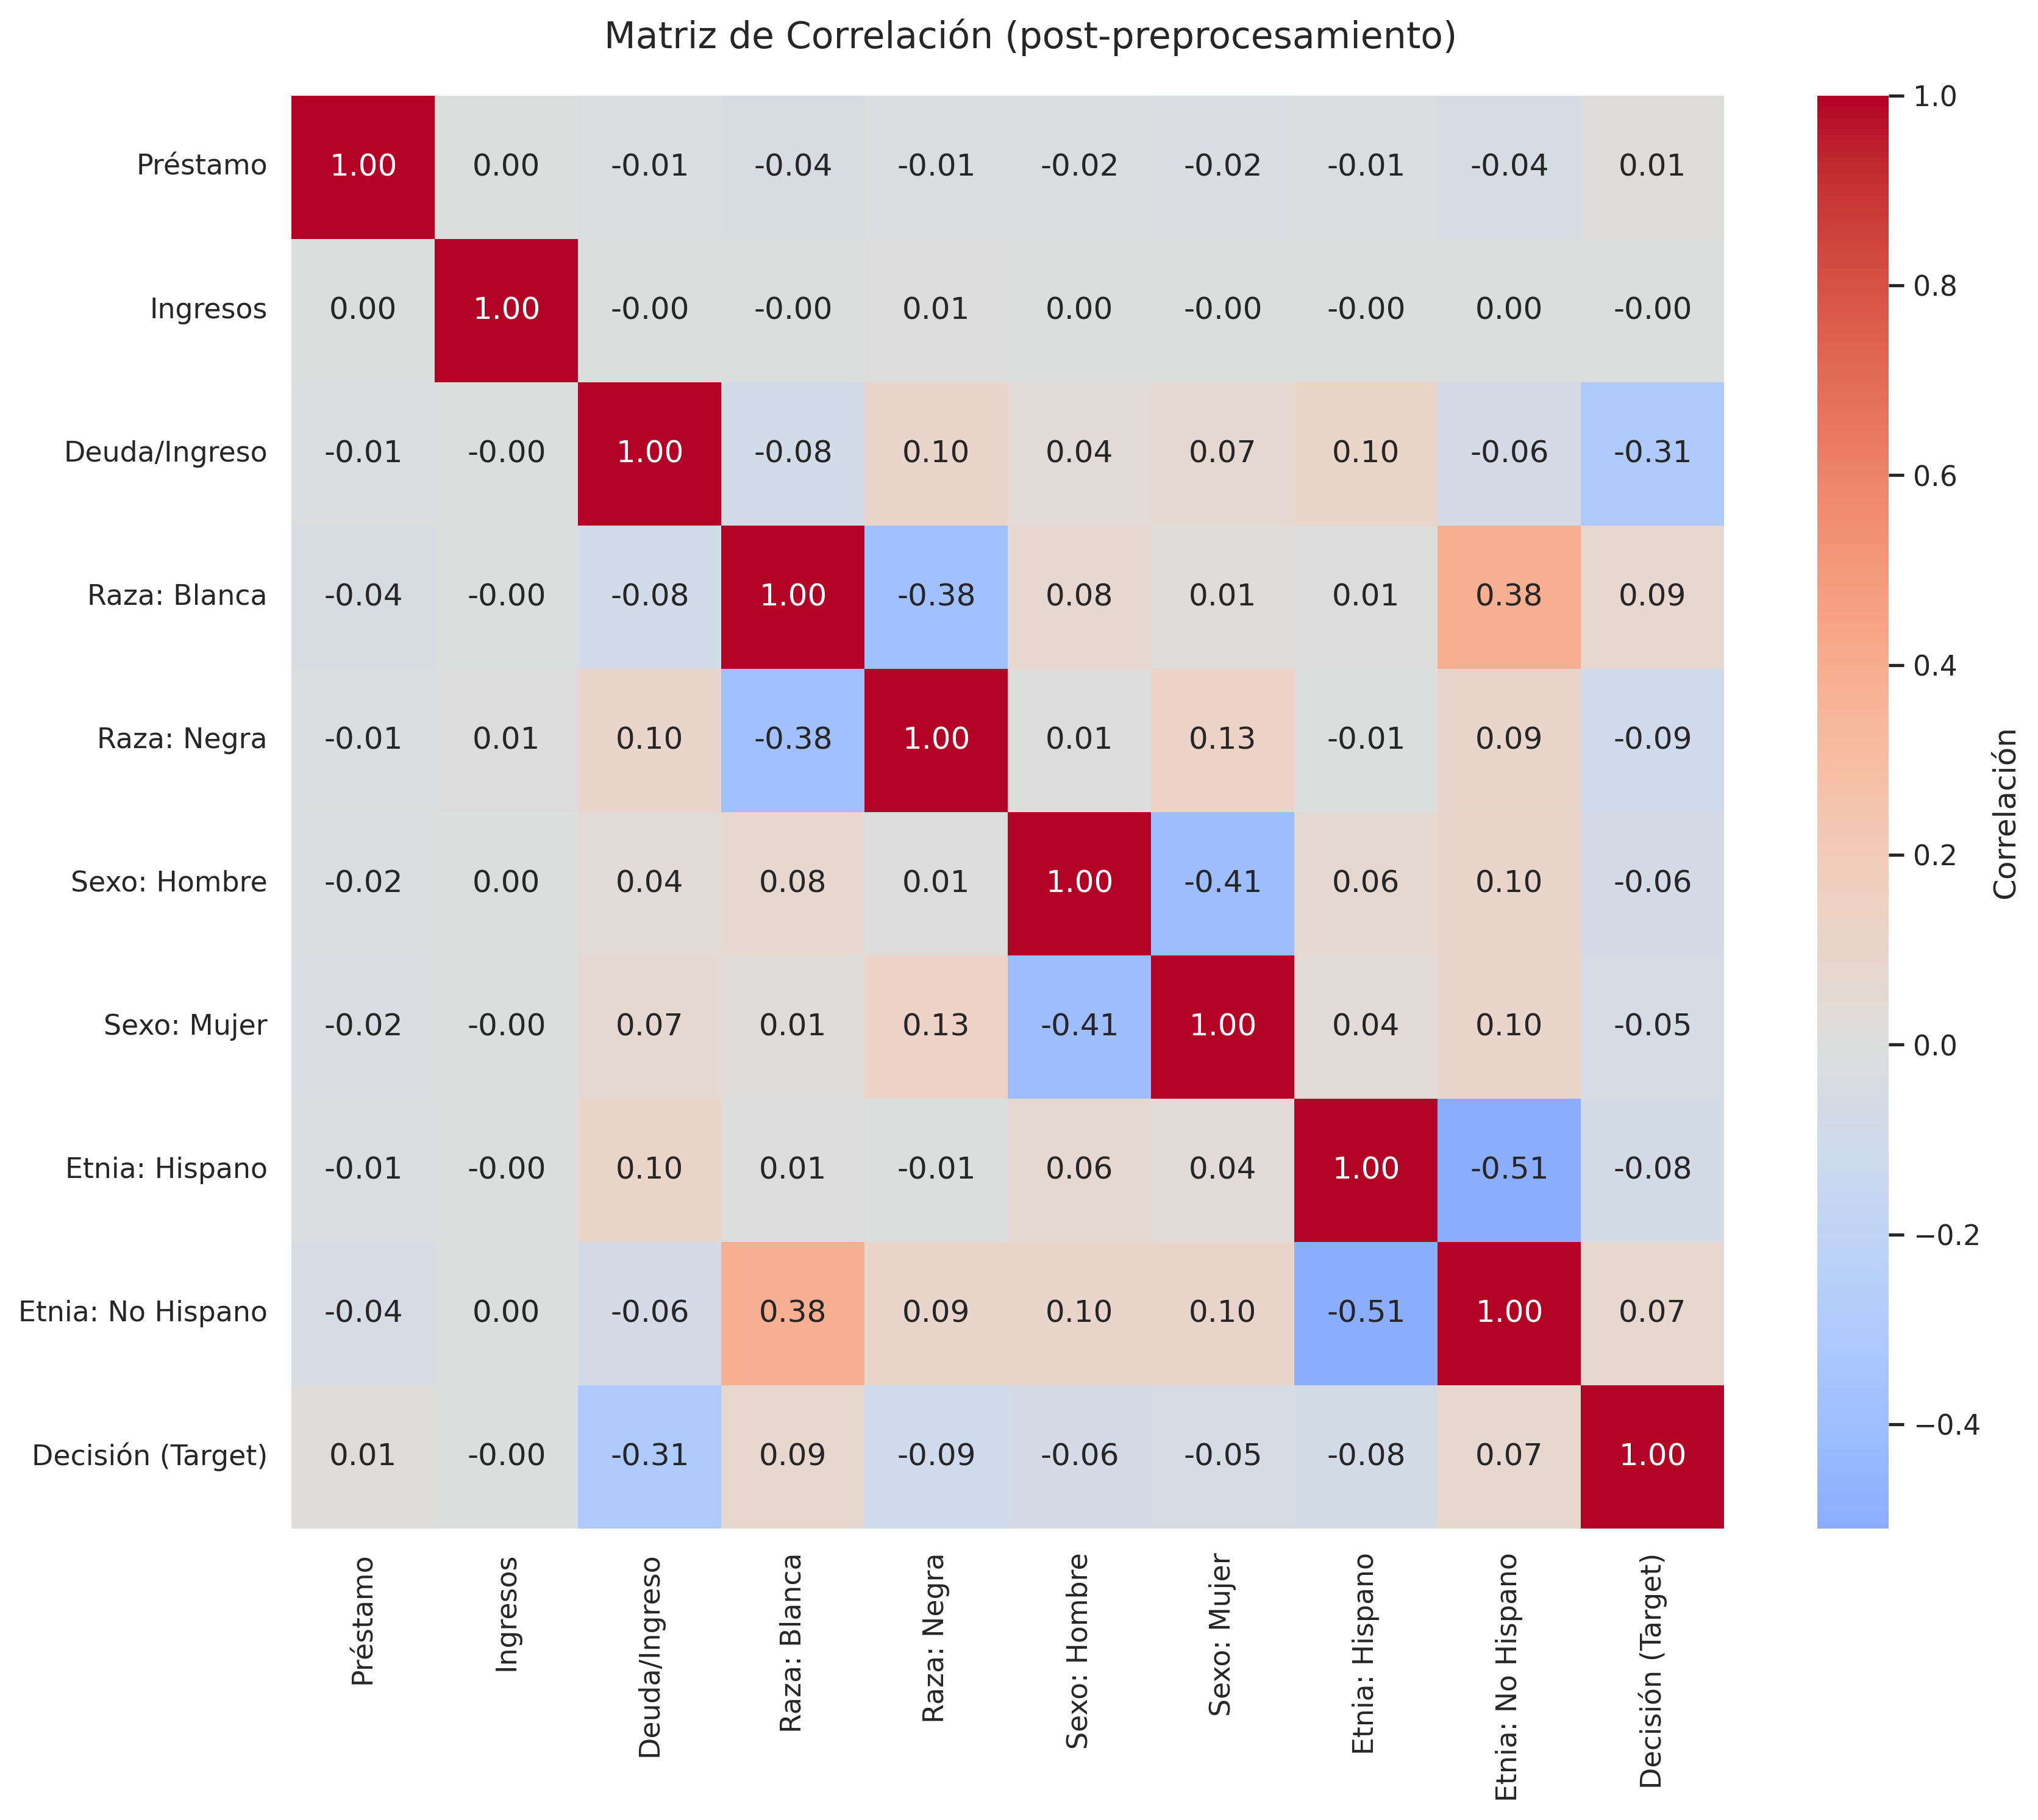
\includegraphics[width=0.75\textwidth]{../outputs/images/2_5_matriz_correlacion_post.png}
\caption{Matriz de correlación post-preprocesamiento. Destacan la correlación negativa de
\texttt{debt\_to\_income\_ratio} ($-0{,}31$) y las correlaciones de los atributos sensibles con el target.}
\label{fig:corr_post}
\end{figure}

\subsection{Preprocesamiento}

\subsubsection{Filtrado de columnas}

Se eliminan dos grupos de columnas antes de cualquier modelado:

\begin{itemize}
    \item \textbf{Identificadores y constantes:} \texttt{activity\_year} (constante, solo 2024),
    \texttt{state\_code} (constante, solo NY), \texttt{lei} (identificador de entidad financiera,
    memorizaría qué bancos aprueban más en vez de aprender el perfil del solicitante) y
    \texttt{census\_tract} (alta cardinalidad, información geográfica ya capturada por \texttt{county\_code}
    y las variables censales).
    \item \textbf{Data leakage:} razones de denegación (\texttt{denial\_reason-*}, solo existen
    tras la decisión negativa), condiciones financieras finales (\texttt{interest\_rate},
    \texttt{rate\_spread}, \texttt{hoepa\_status}, solo existen si se aprueba) y costes de
    formalización (\texttt{total\_loan\_costs}, \texttt{origination\_charges}, etc., son posteriores
    a la decisión). También se excluye \texttt{purchaser\_type} (evento post-concesión).
\end{itemize}

\newpage
\subsubsection{Codificación de variables categóricas}

Se aplican estrategias diferenciadas según el tipo de variable:

\begin{itemize}
    \item \textbf{Numéricas con ``Exempt'':} columnas con valores no numéricos por códigos
    especiales (\texttt{loan\_term}, \texttt{intro\_rate\_period}) se convierten a \texttt{float}
    tratando los no-numéricos como nulos.
    \item \textbf{Variables ordinales:} \texttt{applicant\_age}, \texttt{co-applicant\_age},
    \texttt{debt\_to\_income\_ratio} y \texttt{total\_units} se codifican con mapeo jerárquico
    para preservar el orden (e.g., \texttt{<25}=1, \texttt{25-34}=2, \ldots, \texttt{>74}=7).
    \item \textbf{Variables binarias:} mapeo 0/1 directo, con tratamiento de códigos especiales
    HMDA (1111 = Exempt, 8888 = Not applicable).
    \item \textbf{Variables nominales:} \textit{One-Hot Encoding} sobre \texttt{conforming\_loan\_limit},
    \texttt{derived\_loan\_product\_type}, \texttt{derived\_dwelling\_category},
    \texttt{derived\_ethnicity}, \texttt{derived\_race} y \texttt{derived\_sex}. El dataset pasa
    de 82 a 108 columnas.
\end{itemize}

\subsubsection{Manejo de valores faltantes}

Se elimina toda columna con más del 50\% de valores nulos. Este umbral elimina variables con
vacíos estructurales del formulario HMDA (razas secundarias, sistemas de \textit{scoring} adicionales,
etc.) cuya imputación introduciría ruido inaceptable.

\subsubsection{Partición train/test y pipeline de preprocesamiento}

Se realiza la partición \textbf{antes} del preprocesamiento para evitar \textit{data leakage}: 80\%
entrenamiento (226.665 instancias) y 20\% test (56.667 instancias), estratificada por el target.

El preprocesamiento final se encapsula en un \texttt{Pipeline} de scikit-learn con dos pasos:

\begin{enumerate}
    \item \textbf{Imputación KNN} ($k=5$): equilibrio entre estabilidad y especificidad. Se aplica
    \texttt{fit\_transform} sobre train y \texttt{transform} sobre test.
    \item \textbf{RobustScaler}: elegido frente a \texttt{StandardScaler} por su robustez ante
    los valores atípicos extremos detectados en las variables financieras. Las columnas booleanas
    del OHE se mantienen intactas mediante \texttt{passthrough}.
\end{enumerate}

Las columnas sensibles (\texttt{derived\_race\_*}, \texttt{derived\_sex\_*},
\texttt{derived\_ethnicity\_*}) se conservan en los CSV finales para reconstruir los grupos de
\textit{fairness} en notebooks posteriores sin necesidad de reprocesar el dataset desde cero.

\begin{table}[ht]
\centering
\caption{Resumen del dataset final tras preprocesamiento}
\label{tab:dataset_final}
\small
\begin{tabular}{@{}lcc@{}}
\toprule
\textbf{Conjunto} & \textbf{Instancias} & \textbf{Columnas} \\ \midrule
Train & 226.665 & 81 (80 features + target) \\
Test  & 56.667  & 81 (80 features + target) \\
\bottomrule
\end{tabular}
\end{table}

\newpage
% ============================================================
\section{Metodología}
\label{sec:metodologia}

% ============================================================
\subsection{Modelo Baseline (Notebook 2)}
% ============================================================

\subsubsection{Definición del modelo}

Se entrena un modelo de \textbf{Regresión Logística} como baseline. Al ser el modelo lineal más
simple para clasificación binaria, sirve como referencia para cuantificar la mejora real de los
modelos posteriores, tanto en rendimiento como en equidad. Al igual que en el Notebook~3,
\texttt{FEATURE\_COLS} incluye todas las columnas disponibles del CSV, incluyendo los atributos
sensibles (\texttt{derived\_race\_*}, \texttt{derived\_sex\_*}, \texttt{derived\_ethnicity\_*}).
La diferencia clave respecto al Notebook~3 no es el acceso a los datos sino la capacidad del
modelo: la Regresión Logística solo puede trazar fronteras lineales, por lo que sus métricas de
equidad sirven como referencia de un modelo simple sin restricciones de \textit{fairness}.

\begin{table}[ht]
\centering
\caption{Hiperparámetros del modelo baseline (Regresión Logística)}
\label{tab:baseline_params}
\small
\begin{tabular}{@{}lll@{}}
\toprule
\textbf{Parámetro} & \textbf{Valor} & \textbf{Justificación} \\ \midrule
\texttt{C} & 1.0 & Regularización estándar, sin ajuste \\
\texttt{penalty} & \texttt{'l2'} & Regularización Ridge por defecto \\
\texttt{solver} & \texttt{'lbfgs'} & Adecuado para datasets grandes \\
\texttt{max\_iter} & 1000 & Aumentado para garantizar convergencia \\
\texttt{class\_weight} & \texttt{'balanced'} & Compensa el desbalance $\sim$74/26 \\
\texttt{random\_state} & 42 & Reproducibilidad \\
\bottomrule
\end{tabular}
\end{table}

\subsubsection{Métricas de rendimiento}

\begin{table}[ht]
\centering
\caption{Métricas del modelo baseline --- Regresión Logística}
\label{tab:baseline_metrics}
\small
\begin{tabular}{@{}lccc@{}}
\toprule
\textbf{Modelo} & \textbf{Accuracy} & \textbf{F1-Score} & \textbf{ROC-AUC} \\ \midrule
Regresión Logística (baseline) & 0.7120 & 0.7874 & 0.7697 \\
\bottomrule
\end{tabular}
\end{table}

El modelo baseline alcanza un Accuracy de 0{,}7120 y un ROC-AUC de 0{,}7697, lo que indica
una capacidad discriminativa moderada esperada para un modelo lineal simple con fronteras
de decisión lineales y sin restricciones de \textit{fairness}. El F1-Score de 0{,}7874 sobre la clase mayoritaria contrasta con el
rendimiento sobre denegaciones, reflejando la dificultad de identificar correctamente la clase
negativa a pesar del uso de \texttt{class\_weight='balanced'}. Estos valores constituyen la
referencia de rendimiento sobre la que se medirá la mejora del LightGBM.

\subsubsection{Matriz de confusión y curva ROC}

\begin{figure}[H]
\centering
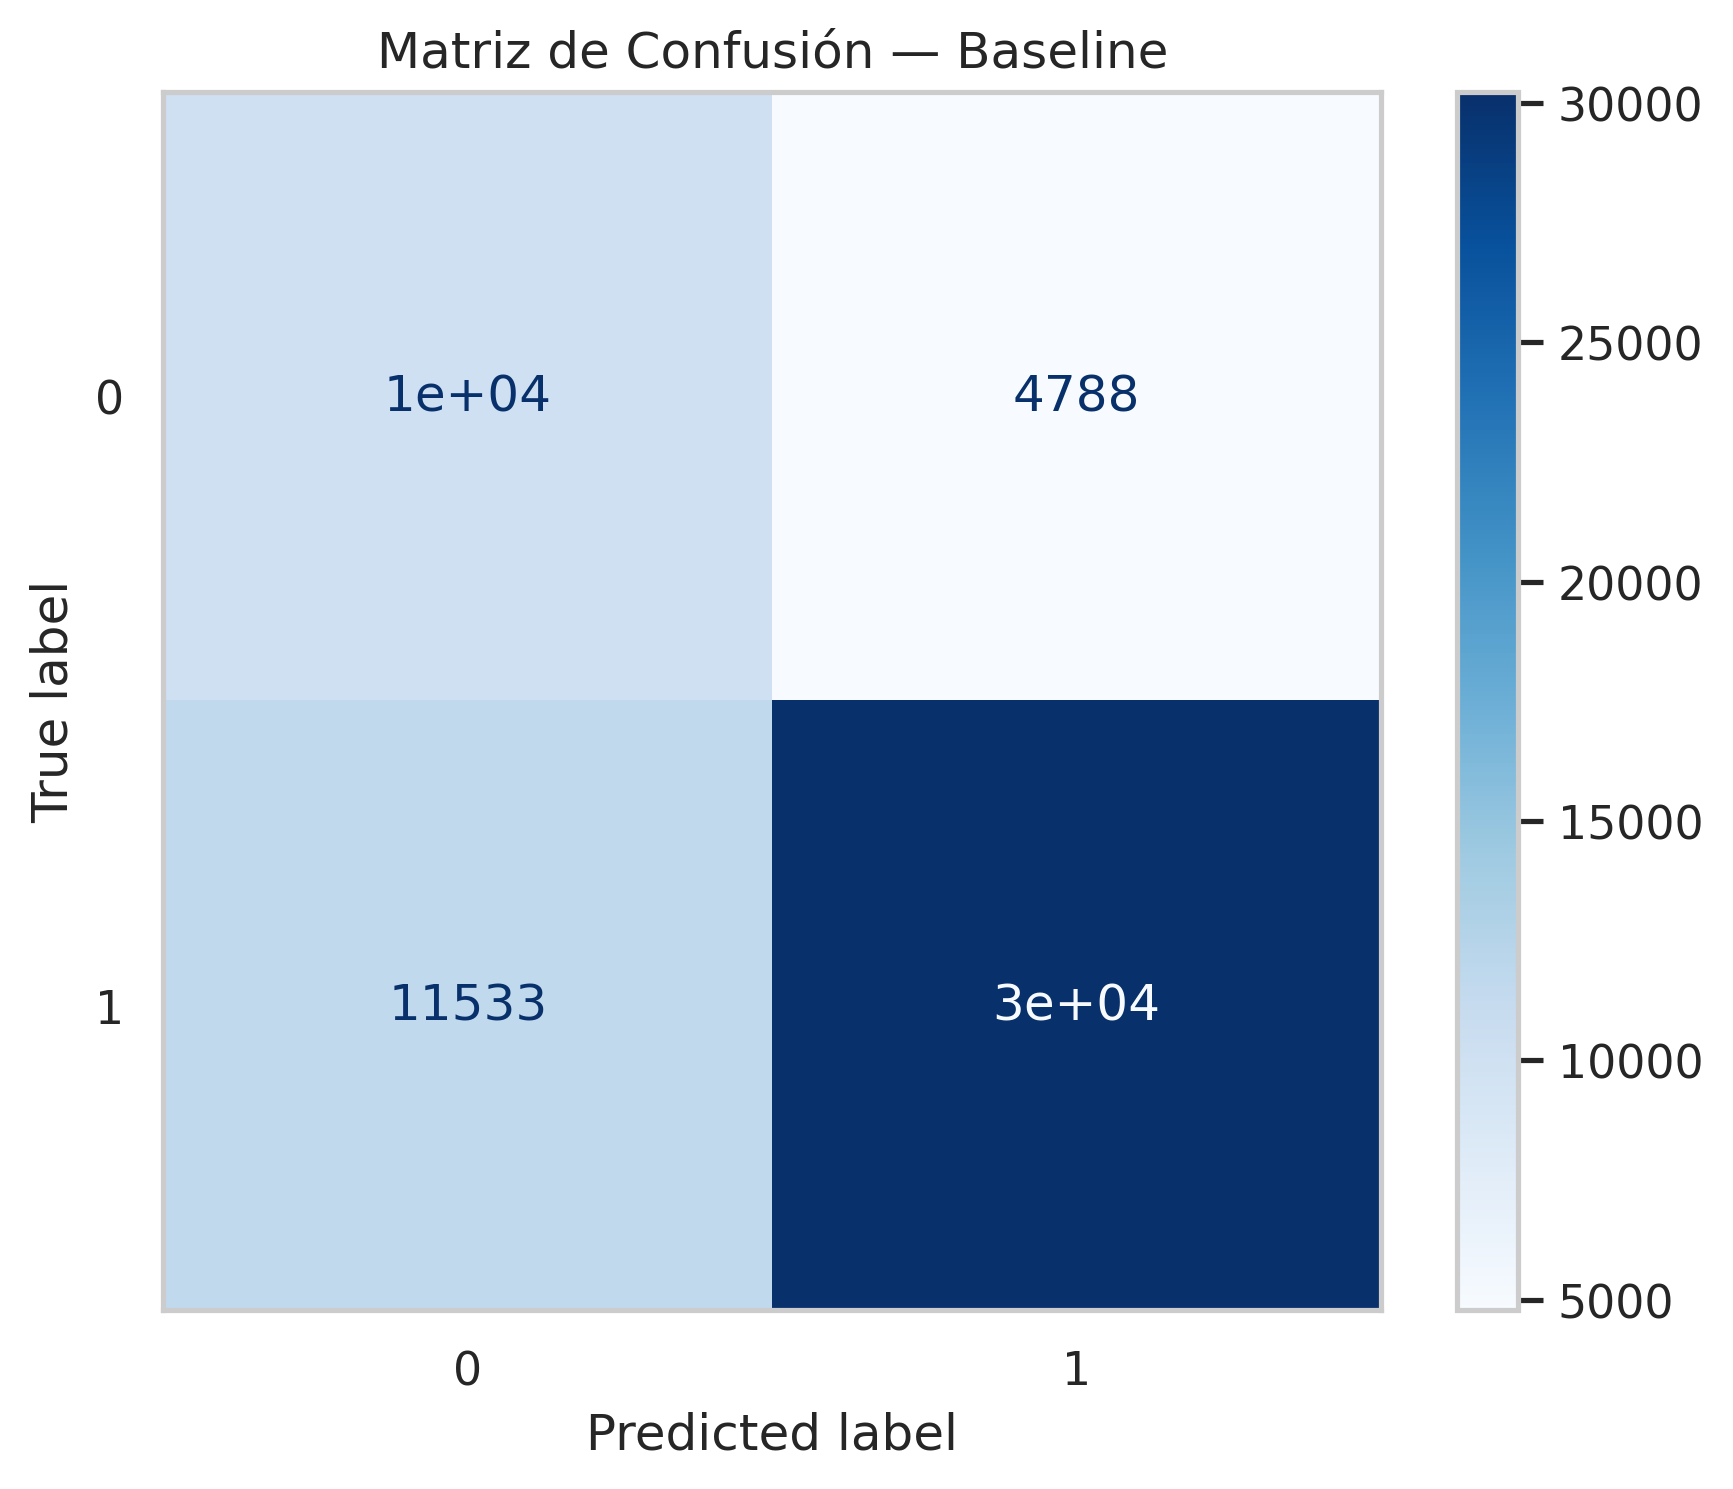
\includegraphics[width=0.5\textwidth]{../outputs/images/matriz_confusion_baseline.png}
\caption{Matriz de confusión --- Regresión Logística (baseline).}
\label{fig:cm_baseline}
\end{figure}

La matriz confirma el desequilibrio en los errores del modelo. De las aprobaciones reales, 11.533
son clasificadas incorrectamente como denegaciones (Falsos Negativos), lo que en el contexto real
implica rechazar solicitudes legítimas de hipoteca. Este tipo de error tiene consecuencias sociales
directas y será uno de los focos del análisis de \textit{fairness} posterior.

\begin{figure}[H]
\centering
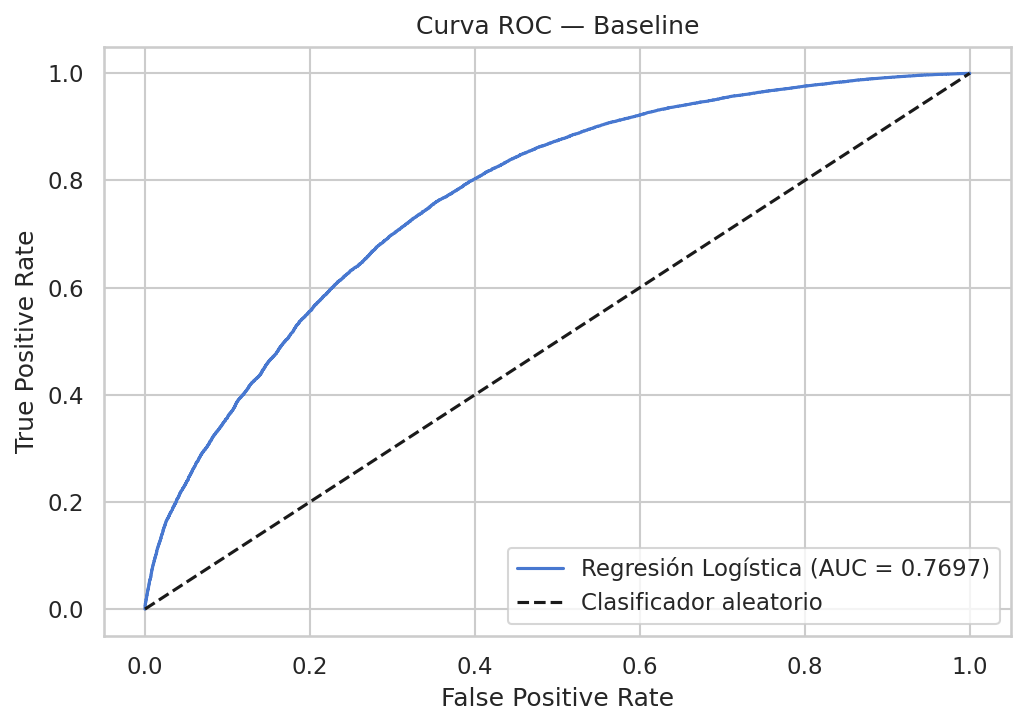
\includegraphics[width=0.55\textwidth]{../outputs/images/curva_roc_baseline.png}
\caption{Curva ROC --- Regresión Logística (baseline). AUC = 0{,}7697.}
\label{fig:roc_baseline}
\end{figure}

\subsubsection{Análisis de Fairness del Baseline}

\begin{figure}[H]
\centering
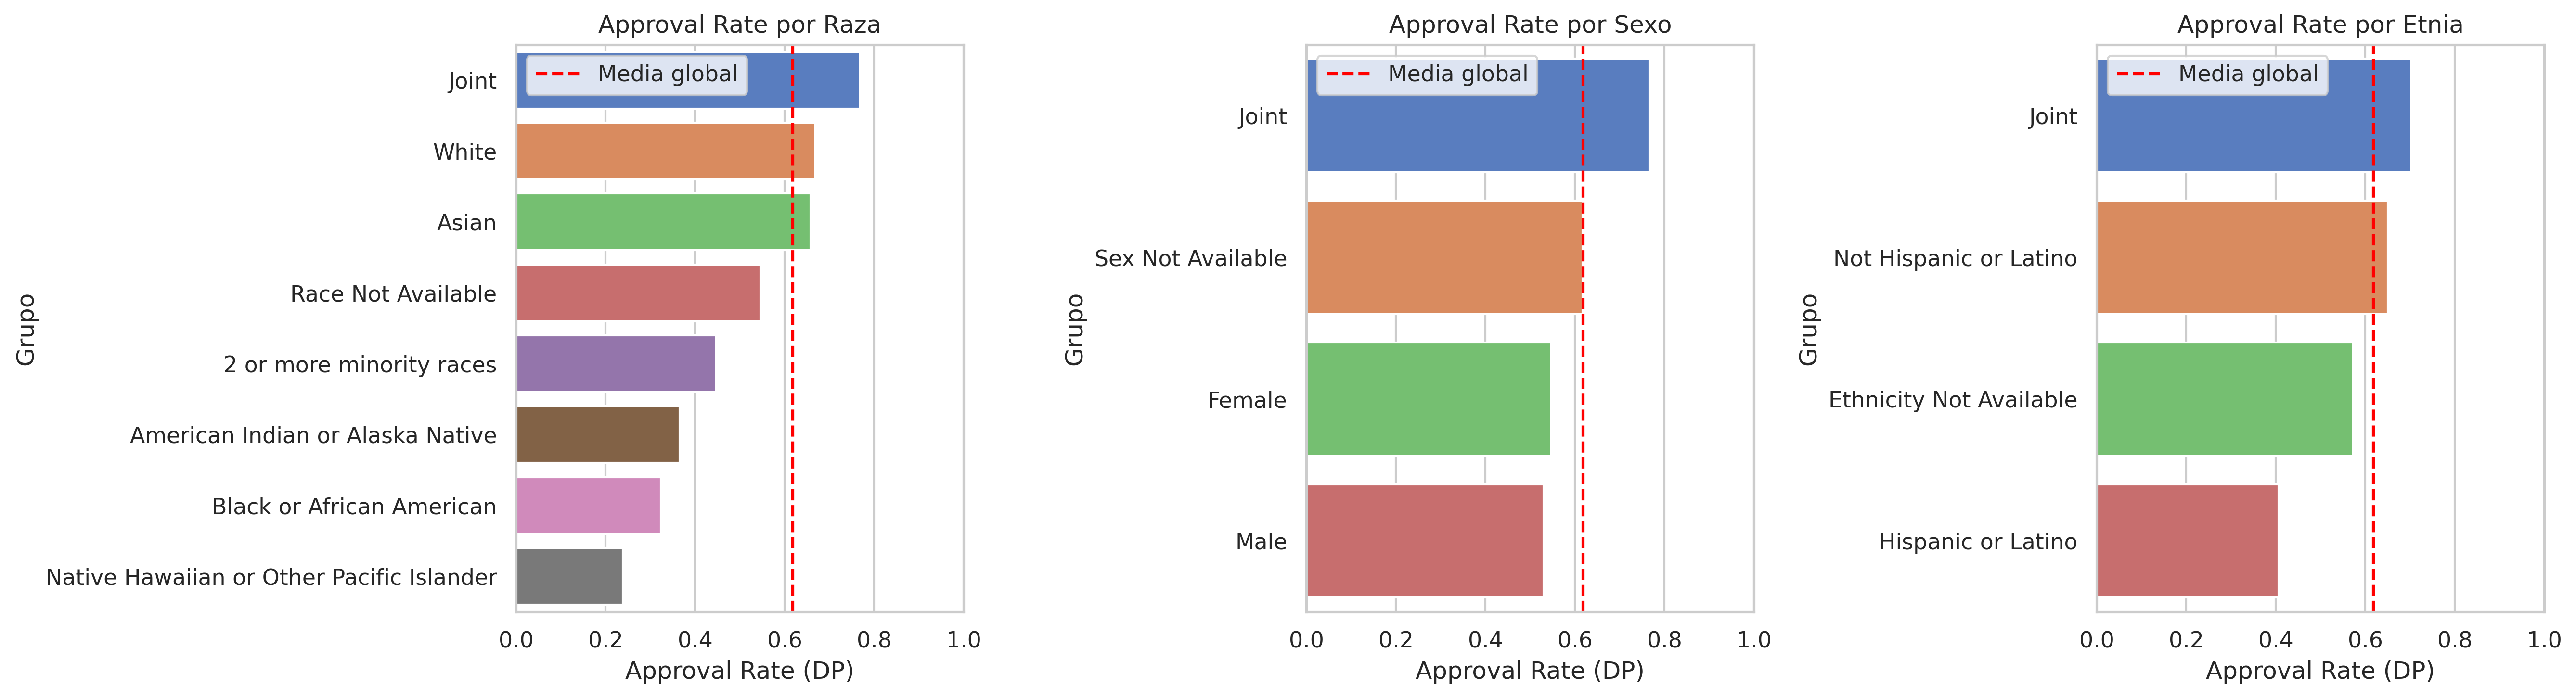
\includegraphics[width=\textwidth]{../outputs/images/fairness_baseline.png}
\caption{Tasas de aprobación por raza, sexo y etnia --- modelo baseline.
La línea roja discontinua marca la media global.}
\label{fig:fairness_baseline}
\end{figure}

\begin{table}[ht]
\centering
\caption{Métricas de fairness del baseline (selección de grupos principales)}
\label{tab:fairness_baseline}
\small
\begin{tabular}{@{}llccc@{}}
\toprule
\textbf{Atributo} & \textbf{Grupo} & \textbf{Approval Rate (DP)} & \textbf{TPR} & \textbf{FPR} \\ \midrule
\multirow{3}{*}{Raza}  & White & 66{,}85\% & 0{,}7595 & 0{,}3803 \\
                        & Black or African American & 32{,}29\% & 0{,}4364 & 0{,}1820 \\
                        & Brecha (pp) & \textbf{34{,}56 pp} & --- & --- \\
\midrule
\multirow{2}{*}{Etnia} & Not Hispanic or Latino & 65{,}00\% & 0{,}7493 & 0{,}3660 \\
                        & Hispanic or Latino & 40{,}61\% & 0{,}5327 & 0{,}2336 \\
\midrule
\multirow{2}{*}{Sexo}  & Joint & 76{,}59\% & 0{,}8559 & 0{,}4679 \\
                        & Female & 54{,}65\% & 0{,}6539 & 0{,}2924 \\
\bottomrule
\end{tabular}
\end{table}

Los resultados revelan diferencias significativas ya en el baseline. La brecha racial entre personas
blancas (66{,}85\%) y negras (32{,}29\%) alcanza los \textbf{34{,}56 pp}, la mayor de los tres
modelos del proyecto. Esto evidencia que incluso un modelo lineal sin restricciones de equidad discrimina
estructuralmente cuando los datos reflejan desigualdades históricas.
Estas métricas establecen la referencia de equidad sobre la que se medirá el impacto de los modelos
posteriores.

\newpage
% ============================================================
\subsection{Modelo Sesgado con XAI (Notebook 3)}
% ============================================================

\subsubsection{Selección del modelo de ensamble}

Para abordar el problema de clasificación binaria se evalúan cuatro modelos de ensamble basados
en árboles: Random Forest, Gradient Boosting, XGBoost y LightGBM. En este notebook se incluyen
\textbf{todas las columnas disponibles como features}, incluyendo los atributos sensibles
(\texttt{derived\_race\_*}, \texttt{derived\_sex\_*}, \texttt{derived\_ethnicity\_*}). El objetivo
es evaluar el comportamiento natural de los modelos de ensamble sin restricciones, para identificar
el sesgo inherente que introducen cuando tienen acceso a información demográfica.

Se descarta el uso de SVM por su inasumible coste computacional frente a matrices dispersas de
este tamaño, y de Árboles de Decisión individuales por su tendencia al sobreajuste.

\paragraph{Comparativa de modelos.}

La optimización de hiperparámetros se realiza mediante \texttt{GridSearchCV} con validación cruzada
de 3 \textit{folds} y \texttt{roc\_auc} como métrica de optimización (estándar en la industria
financiera para problemas de clasificación con desbalance).

\begin{table}[ht]
\centering
\caption{Comparativa de modelos de ensamble (mejor configuración de cada familia)}
\label{tab:comparativa_modelos}
\small
\begin{tabular}{@{}lccccc@{}}
\toprule
\textbf{Modelo} & \textbf{Accuracy} & \textbf{F1-Score} & \textbf{ROC-AUC} & \textbf{Tiempo (s)} \\ \midrule
Baseline (Regresión Logística) & 0{,}7120 & 0{,}7874 & 0{,}7694 & --- \\
Random Forest                  & 0{,}8572 & 0{,}9067 & 0{,}8792 & $\sim$120 \\
Gradient Boosting              & 0{,}8619 & 0{,}9113 & 0{,}8871 & $\sim$320 \\
XGBoost                        & 0{,}8612 & 0{,}9110 & 0{,}8864 & $\sim$45  \\
\textbf{LightGBM}              & \textbf{0{,}8621} & \textbf{0{,}9116} & \textbf{0{,}8868} & \textbf{1{,}90} \\
\bottomrule
\end{tabular}
\end{table}

\begin{table}[ht]
\centering
\caption{Hiperparámetros óptimos del LightGBM tras GridSearchCV (108 combinaciones, 3 folds)}
\label{tab:lgbm_params}
\small
\begin{tabular}{@{}ll@{}}
\toprule
\textbf{Parámetro} & \textbf{Valor óptimo} \\ \midrule
\texttt{learning\_rate} & 0.1 \\
\texttt{max\_depth}     & 7 \\
\texttt{n\_estimators}  & 200 \\
\texttt{num\_leaves}    & 127 \\
\texttt{subsample}      & 0.8 \\
\bottomrule
\end{tabular}
\end{table}

\textbf{LightGBM se selecciona como modelo ganador} por su combinación óptima de rendimiento
y eficiencia computacional. Con un ROC-AUC de 0{,}8868 prácticamente idéntico al Gradient
Boosting (0{,}8871), lo logra en apenas 1{,}90 segundos frente a los $\sim$320 del GB. Esta
diferencia de dos órdenes de magnitud en tiempo justifica la elección, especialmente en un contexto
de optimización posterior con Fairlearn.

\begin{discusion}
\discusiontitle
LightGBM construye los árboles por hojas (\textit{leaf-wise}) en lugar de por niveles
(\textit{level-wise}) como el GB estándar. Esto lo hace significativamente más rápido y preciso
en datasets grandes, a costa de ser más propenso al sobreajuste si no se controla \texttt{num\_leaves}.
Los nombres de columnas se limpian previamente (sustitución de caracteres especiales por guiones
bajos) porque LightGBM no soporta caracteres como \texttt{:}, \texttt{,} o \texttt{[]} en los
nombres de features.
\end{discusion}

\subsubsection{Métricas de rendimiento}

\begin{figure}[H]
\centering
\includegraphics[width=0.85\textwidth]{../outputs/images/curva_roc_modelos.png}
\caption{Curvas ROC comparativas --- todos los modelos evaluados en el Notebook 3.}
\label{fig:roc_modelos}
\end{figure}

\begin{figure}[H]
\centering
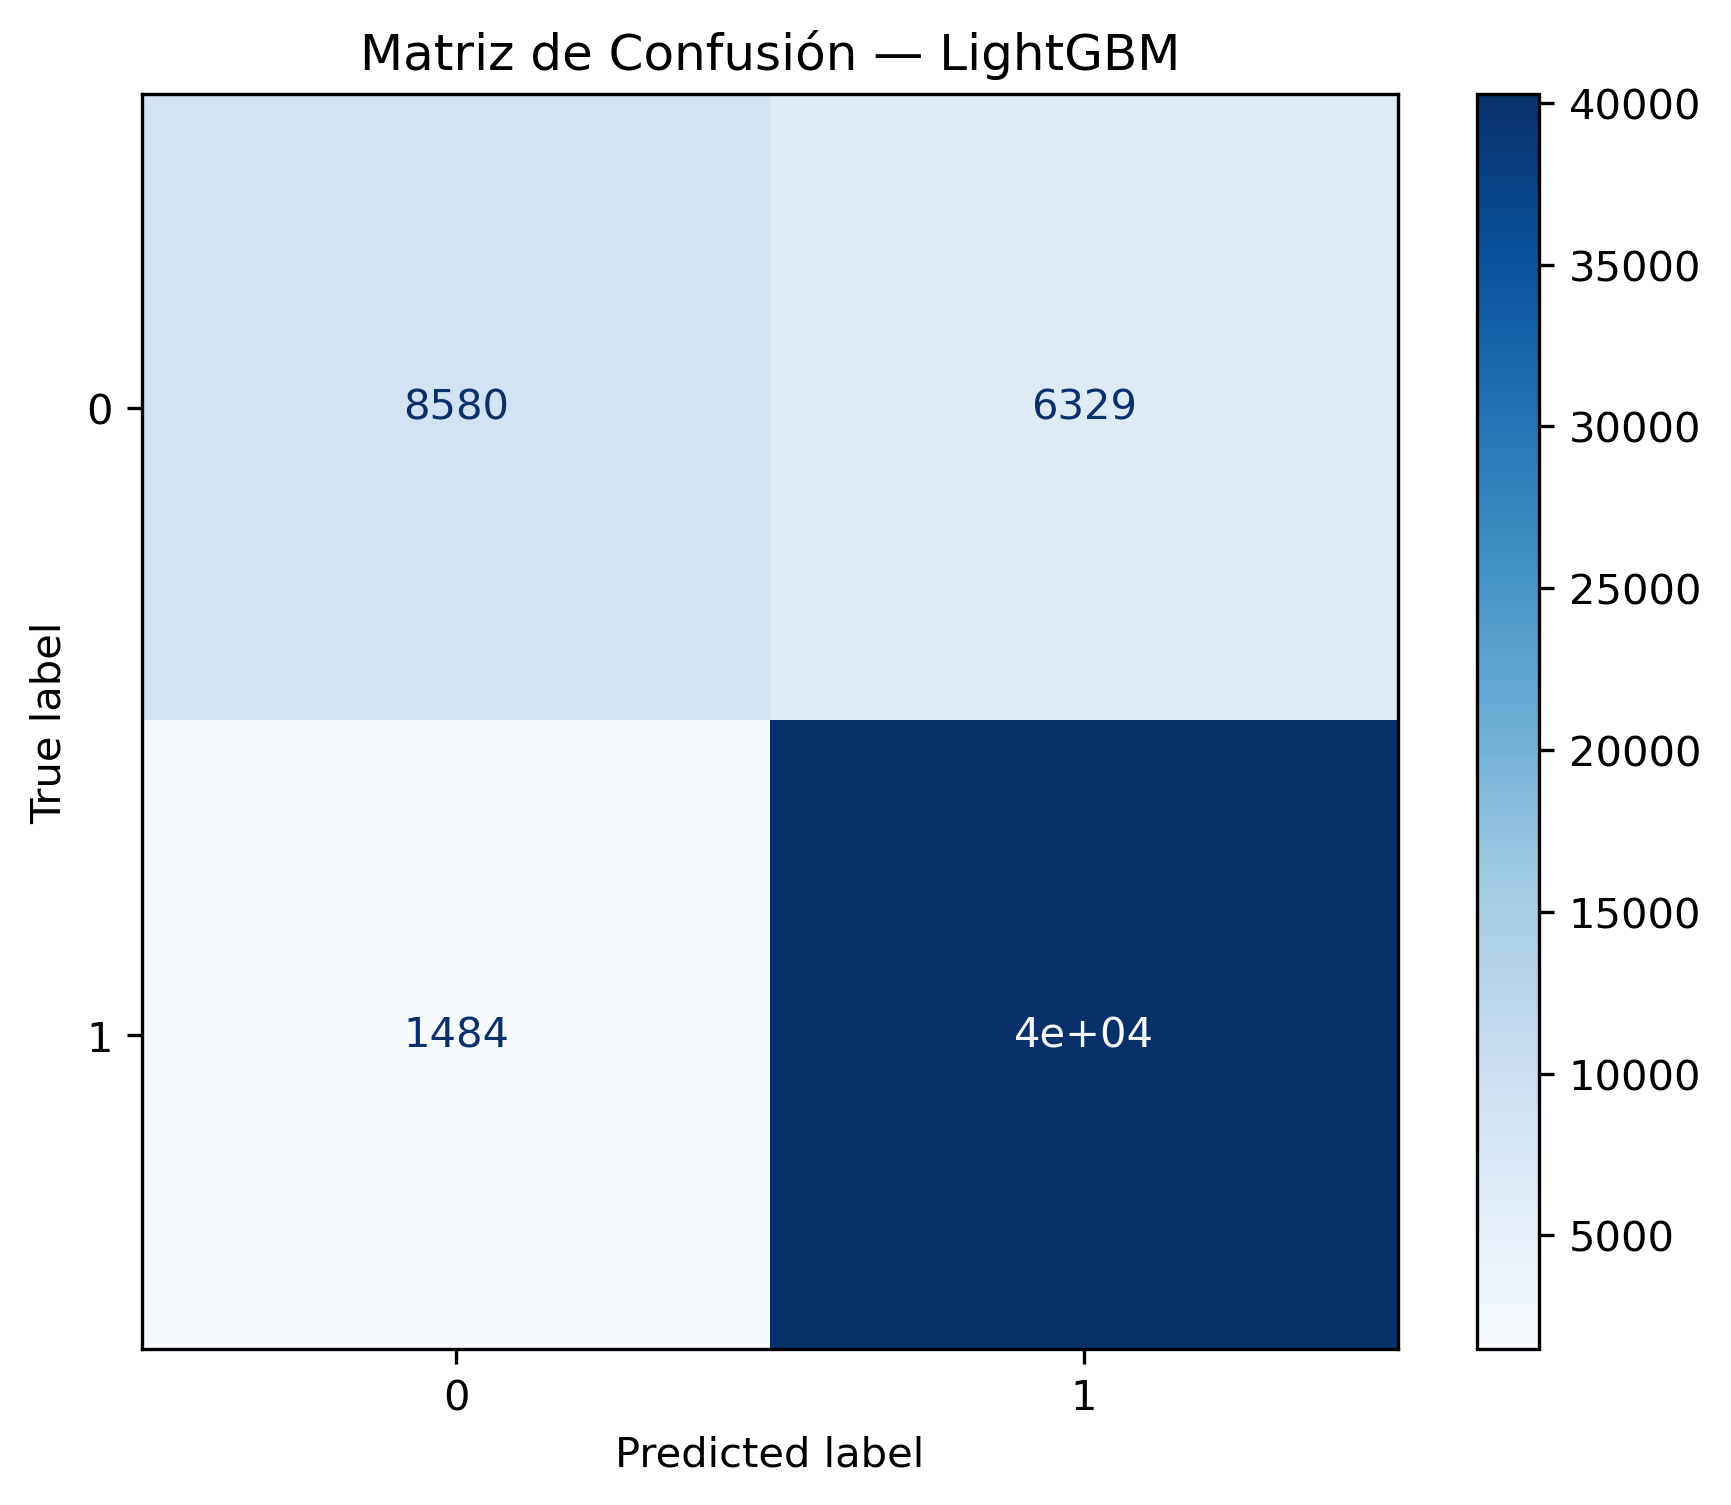
\includegraphics[width=0.65\textwidth]{../outputs/images/matriz_confusion_lgbm.png}
\caption{Matriz de confusión --- LightGBM sesgado (modelo ganador).}
\label{fig:cm_lgbm}
\end{figure}

\subsubsection{Análisis de Fairness del modelo sesgado}

\begin{figure}[H]
\centering
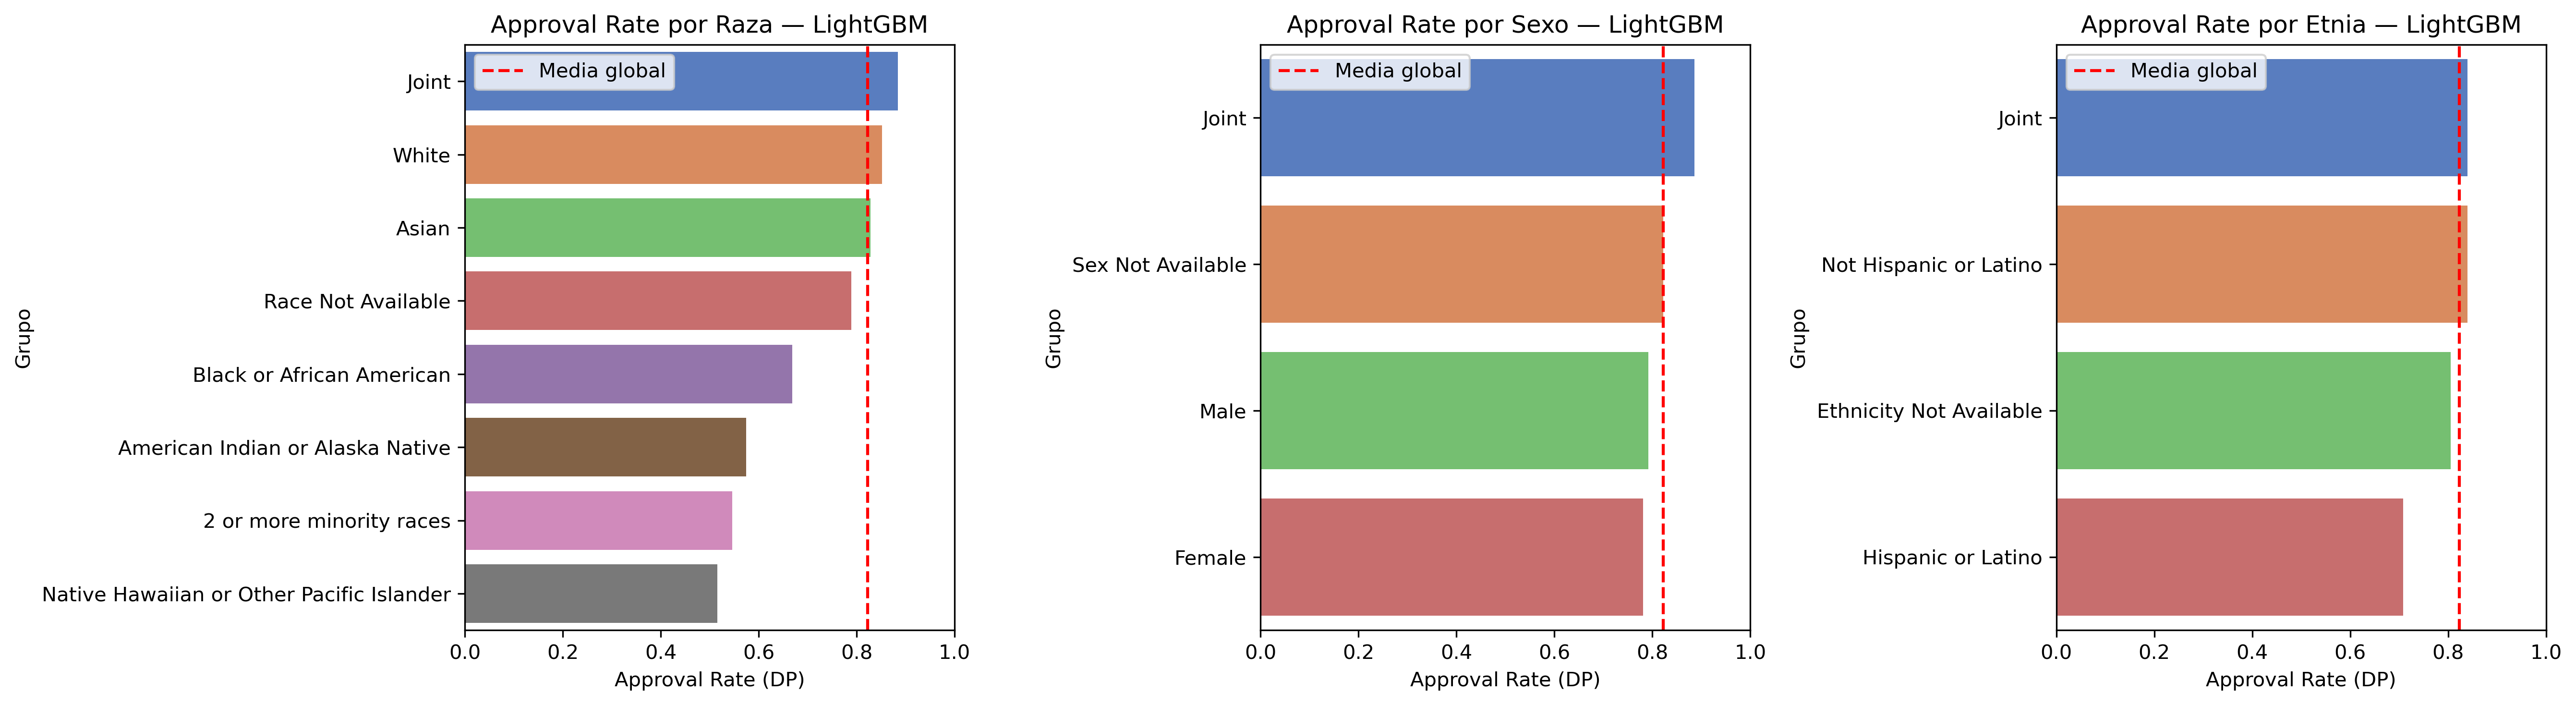
\includegraphics[width=\textwidth]{../outputs/images/fairness_lgbm.png}
\caption{Tasas de aprobación por raza, sexo y etnia --- LightGBM sesgado.}
\label{fig:fairness_lgbm}
\end{figure}

\begin{table}[ht]
\centering
\caption{Métricas de fairness --- LightGBM sesgado (selección de grupos principales)}
\label{tab:fairness_lgbm}
\small
\begin{tabular}{@{}llccc@{}}
\toprule
\textbf{Atributo} & \textbf{Grupo} & \textbf{Approval Rate (DP)} & \textbf{TPR} & \textbf{FPR} \\ \midrule
\multirow{3}{*}{Raza}  & White & 85{,}25\% & 0{,}9709 & 0{,}4648 \\
                        & Black or African American & 66{,}86\% & 0{,}9189 & 0{,}3166 \\
                        & Brecha (pp) & \textbf{18{,}39 pp} & --- & --- \\
\midrule
\multirow{2}{*}{Etnia} & Not Hispanic or Latino & 83{,}92\% & 0{,}9685 & 0{,}4422 \\
                        & Hispanic or Latino & 70{,}78\% & 0{,}9333 & 0{,}3166 \\
\midrule
\multirow{2}{*}{Sexo}  & Joint & 88{,}63\% & 0{,}9764 & 0{,}5101 \\
                        & Female & 78{,}06\% & 0{,}9553 & 0{,}3751 \\
\bottomrule
\end{tabular}
\end{table}

LightGBM reduce la brecha racial respecto al baseline (de 34{,}56 pp a 18{,}39 pp) como
\textbf{efecto secundario de un mejor ajuste global}, no por diseño. El modelo sigue utilizando
activamente la raza para tomar decisiones, tal como confirma el análisis SHAP de la siguiente
sección. La brecha étnica (13{,}14 pp) y la de sexo (diferencias de $\sim$10 pp) también persisten.

\subsubsection{Explicabilidad con SHAP}

\begin{figure}[H]
\centering
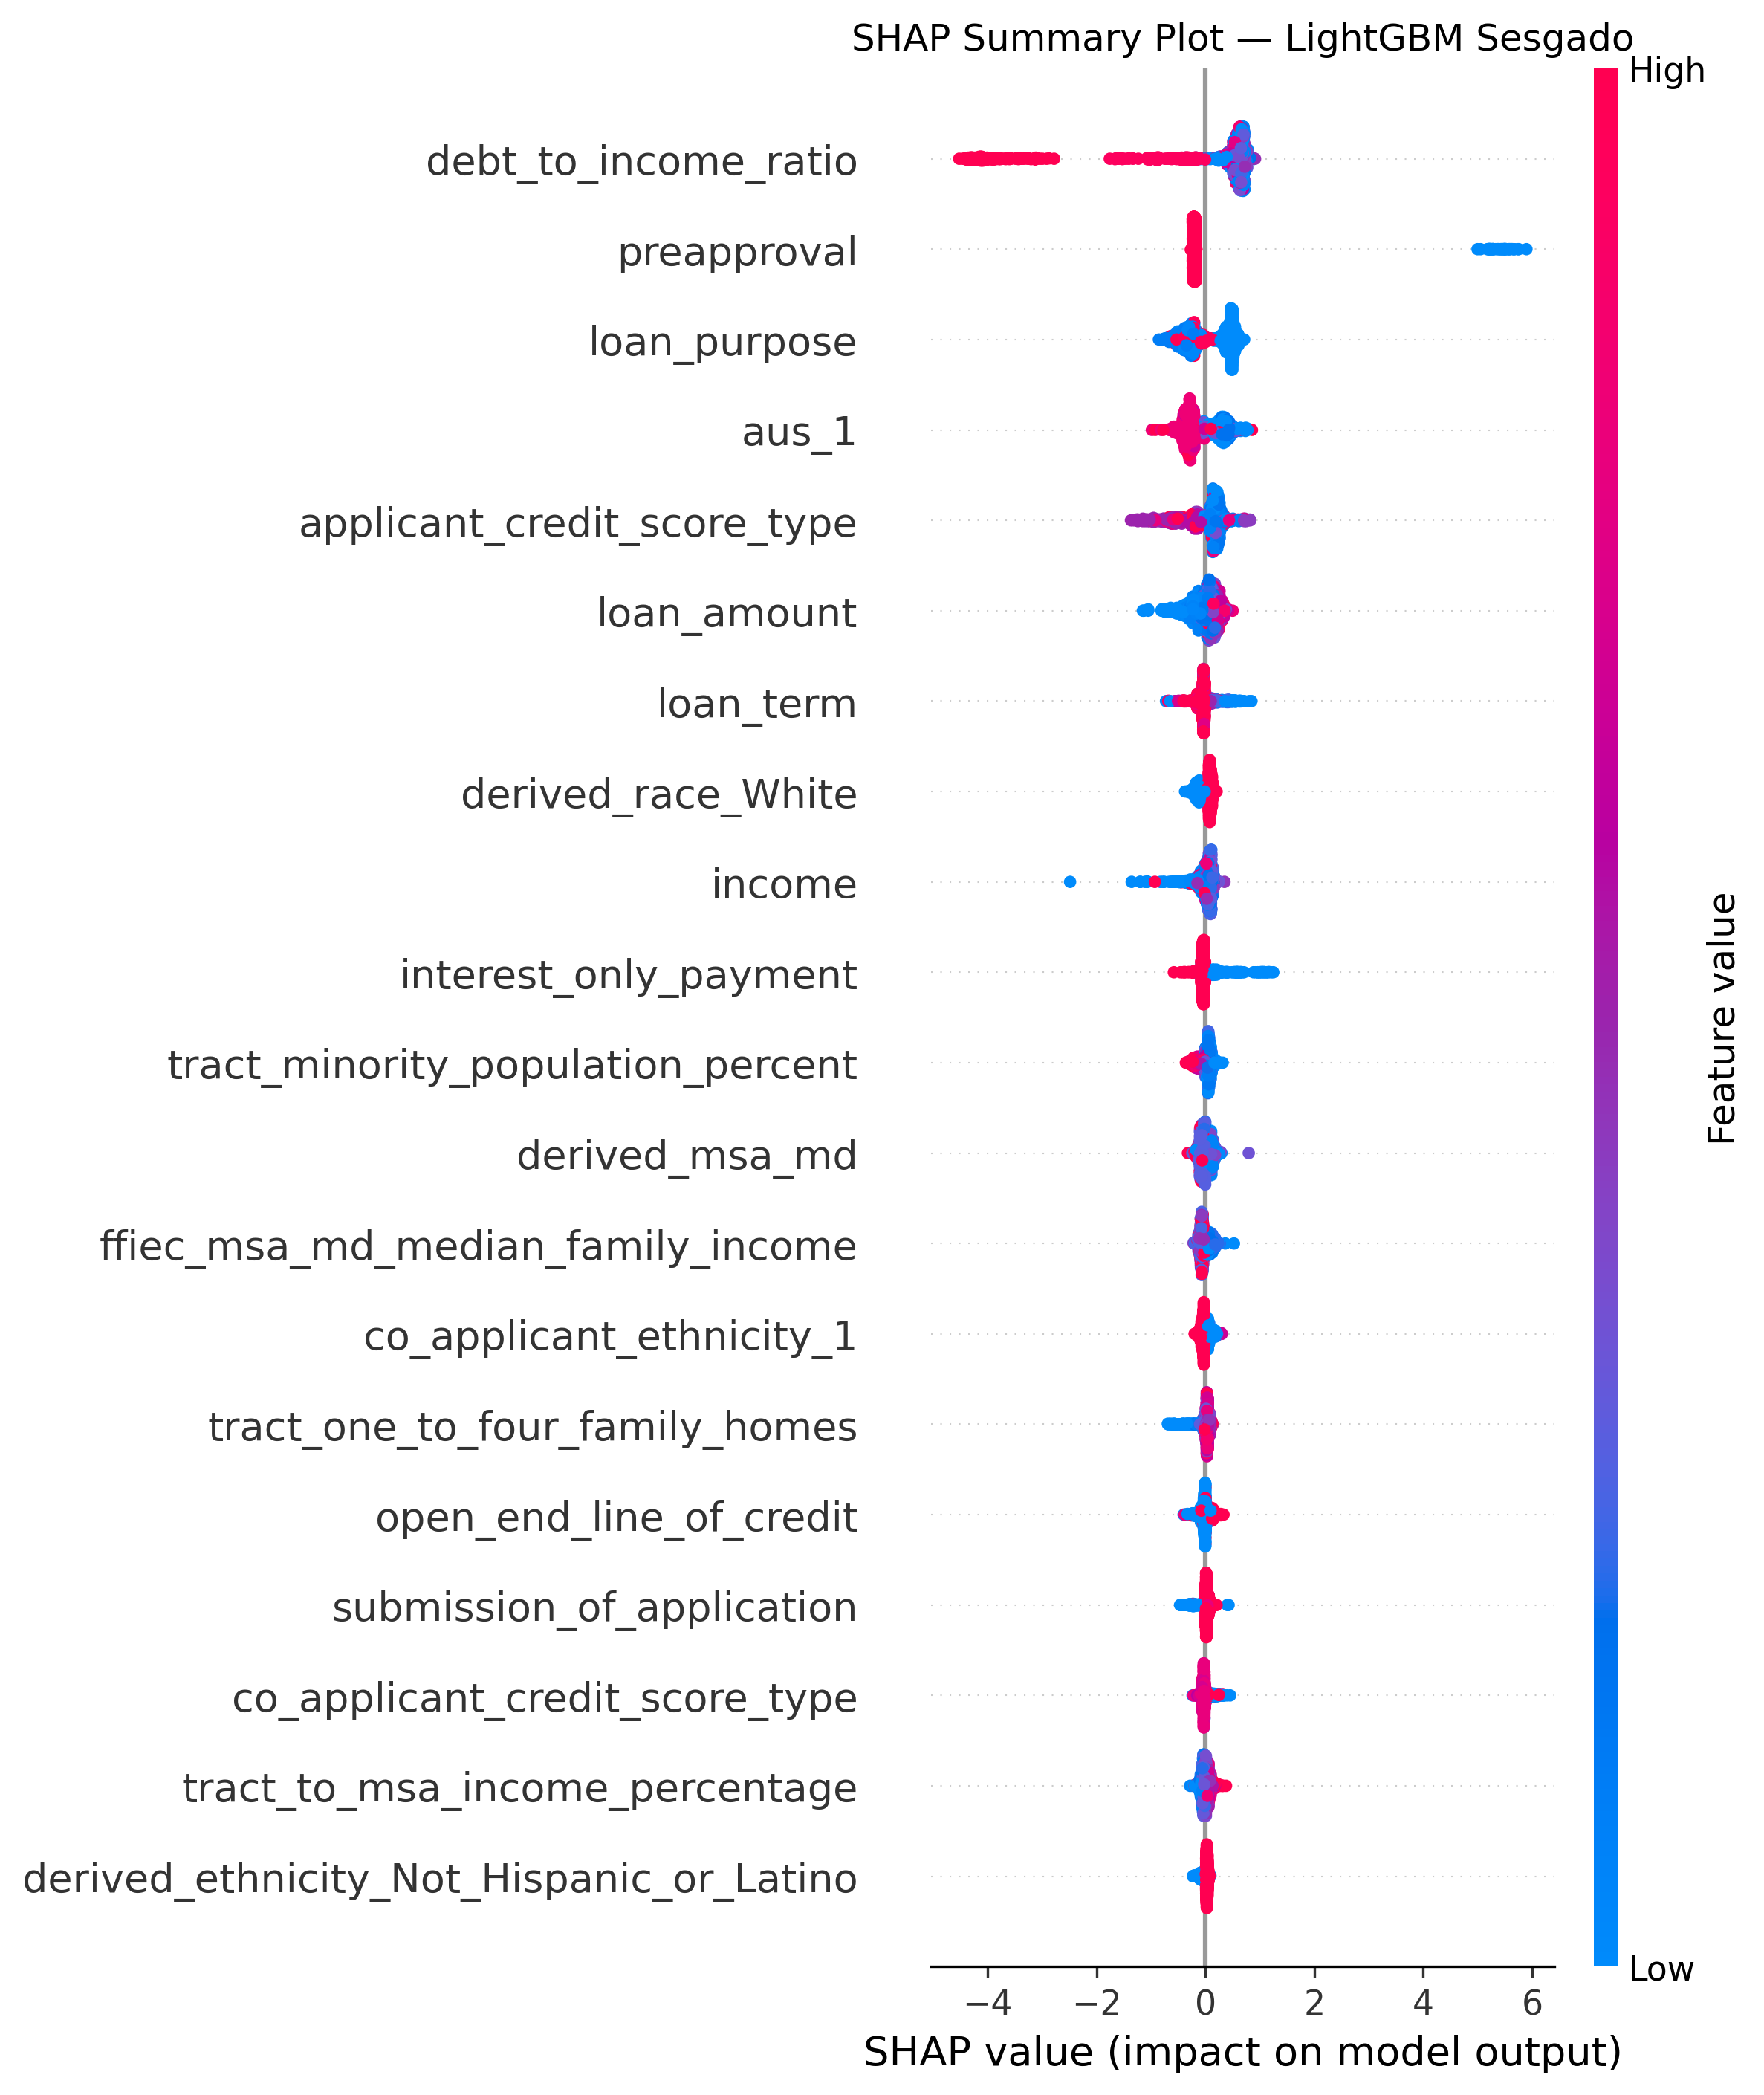
\includegraphics[width=\textwidth]{../outputs/images/shap_summary_sesgado.png}
\caption{SHAP Summary Plot --- LightGBM sesgado. Cada punto representa una instancia del
conjunto de test. El color indica el valor de la feature (rojo = alto, azul = bajo).}
\label{fig:shap_summary_lgbm}
\end{figure}

\begin{figure}[H]
\centering
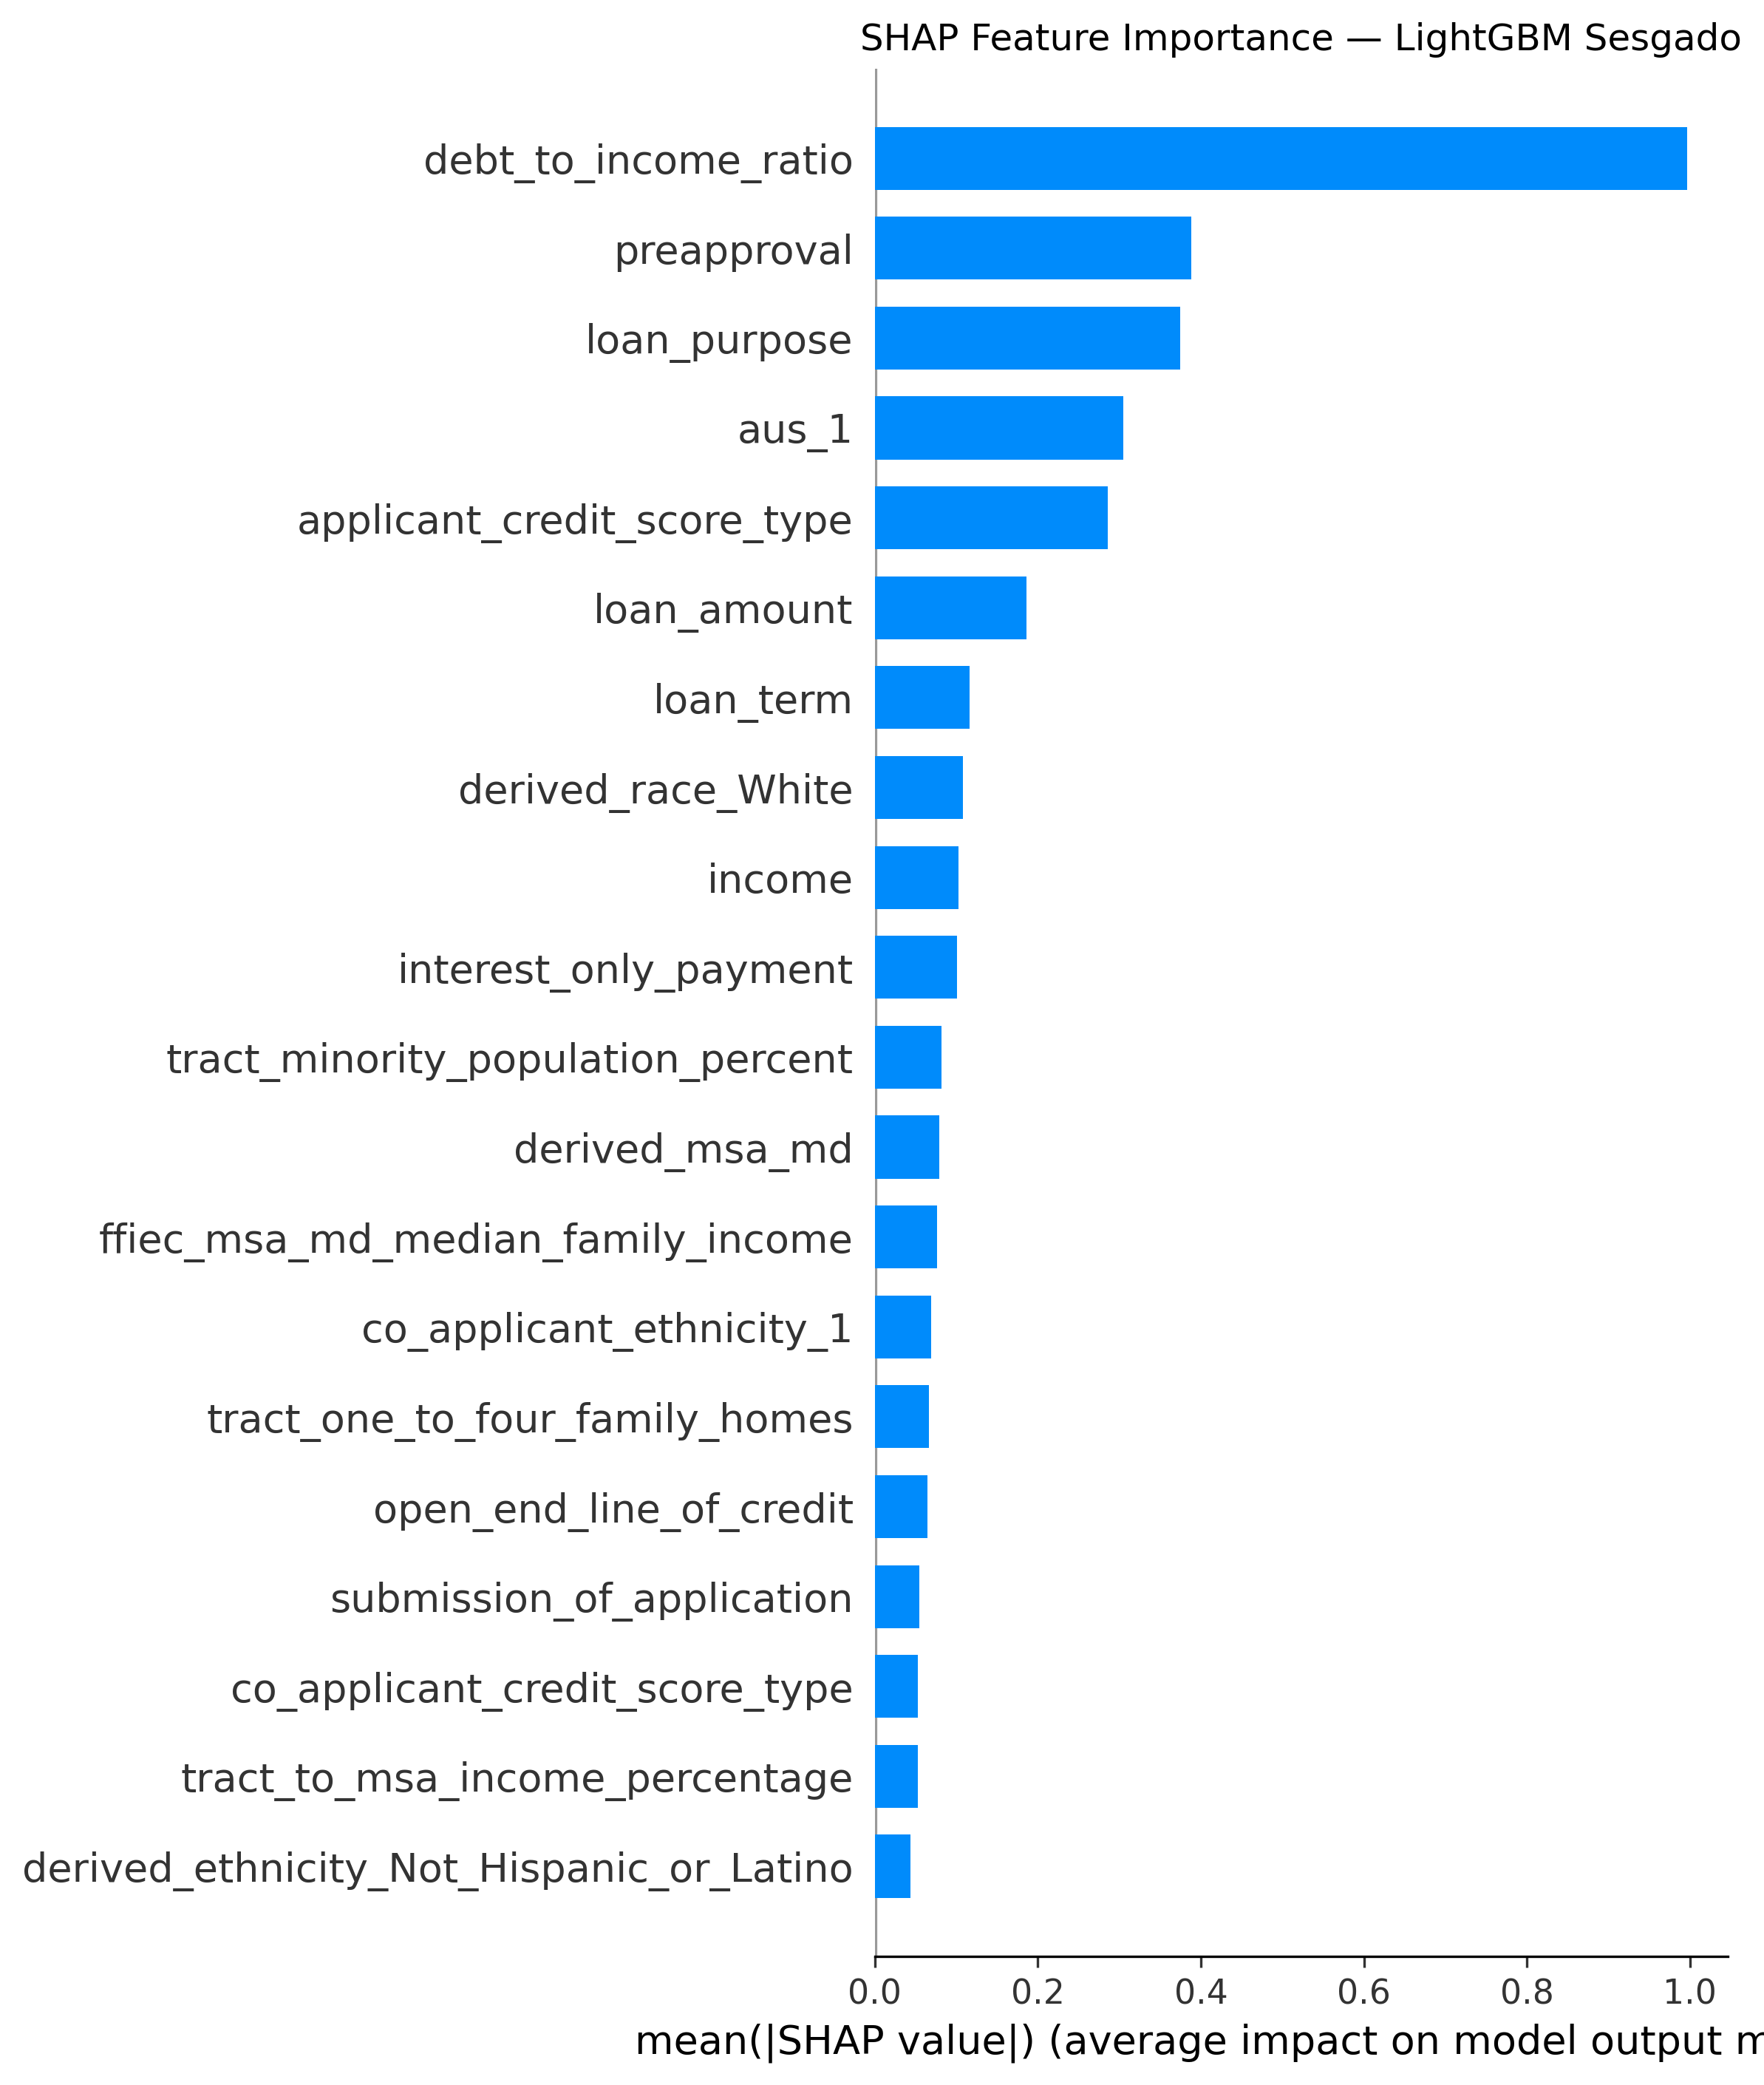
\includegraphics[width=\textwidth]{../outputs/images/shap_bar_sesgado.png}
\caption{SHAP Feature Importance (importancia media absoluta) --- LightGBM sesgado.
En rojo, las features sensibles (raza, sexo, etnia).}
\label{fig:shap_bar_lgbm}
\end{figure}

El análisis SHAP revela que \texttt{debt\_to\_income\_ratio} domina absolutamente las predicciones
del modelo, seguido de \texttt{preapproval}, \texttt{loan\_purpose} y \texttt{aus\_1}. Lo más
relevante para el análisis de sesgo es la posición de \textbf{\texttt{derived\_race\_White}}:
aparece en la \textbf{posición 8} del ranking global con una importancia media absoluta de
$\sim$0{,}10. Esto confirma que el modelo sesgado utiliza activamente la raza del solicitante para
tomar decisiones, con valores altos de \texttt{derived\_race\_White} empujando hacia la aprobación.
Este resultado justifica la necesidad de aplicar técnicas de mitigación en el Notebook~4.

\newpage
% ============================================================
\subsection{Modelo Mitigado con XAI (Notebook 4)}
% ============================================================

\subsubsection{Técnica de mitigación: ExponentiatedGradient}

Se aplica \texttt{ExponentiatedGradient} de Fairlearn sobre el LightGBM optimizado del
Notebook~3, usando \texttt{EqualizedOdds} como restricción de equidad. Esta técnica entrena
iterativamente múltiples versiones del modelo base con distintos pesos por muestra, buscando
el punto óptimo en el que las tasas de error (TPR y FPR) se igualen entre el grupo
\texttt{derived\_race\_White} y el resto.

\begin{discusion}
\discusiontitle
El atributo sensible principal es \texttt{derived\_race\_White} porque es donde se concentra
el mayor sesgo del modelo (posición 8 en SHAP, brecha de 18{,}39 pp). Se usa
\texttt{sample\_weight\_name='sample\_weight'} para integrar correctamente LightGBM con
Fairlearn. Las predicciones del modelo mitigado se obtienen con \texttt{\_pmf\_predict} en lugar
de \texttt{predict\_proba}, ya que Fairlearn combina internamente varios predictores ponderados
y no expone directamente un método estándar de probabilidades. Los valores SHAP se calculan
sobre la media ponderada (\texttt{predictors\_} y \texttt{weights\_}) para obtener una
explicabilidad representativa del ensemble mitigado.
\end{discusion}

\subsubsection{Métricas de rendimiento comparativas}

\begin{table}[ht]
\centering
\caption{Comparativa de rendimiento --- LightGBM sesgado vs.\ mitigado}
\label{tab:rendimiento_mitigado}
\small
\begin{tabular}{@{}lccc@{}}
\toprule
\textbf{Modelo} & \textbf{Accuracy} & \textbf{F1-Score} & \textbf{ROC-AUC} \\ \midrule
LightGBM Sesgado  & 0{,}8621 & 0{,}9116 & 0{,}8868 \\
LightGBM Mitigado & 0{,}8622 & 0{,}9117 & \textbf{0{,}7803} \\
\bottomrule
\end{tabular}
\end{table}

La mitigación apenas afecta a las métricas globales de clasificación: Accuracy y F1-Score son
prácticamente idénticos entre el modelo sesgado y el mitigado, con diferencias inferiores a 0{,}001.
Sin embargo, el \textbf{ROC-AUC cae de 0{,}8868 a 0{,}7803}, una reducción de $\sim$10{,}6 pp.
Esta divergencia refleja que el modelo mitigado mantiene una capacidad de clasificación directa
similar pero pierde poder discriminativo en el ordenamiento de probabilidades, precisamente donde
la restricción de equidad actúa con más fuerza.

\begin{figure}[H]
\centering
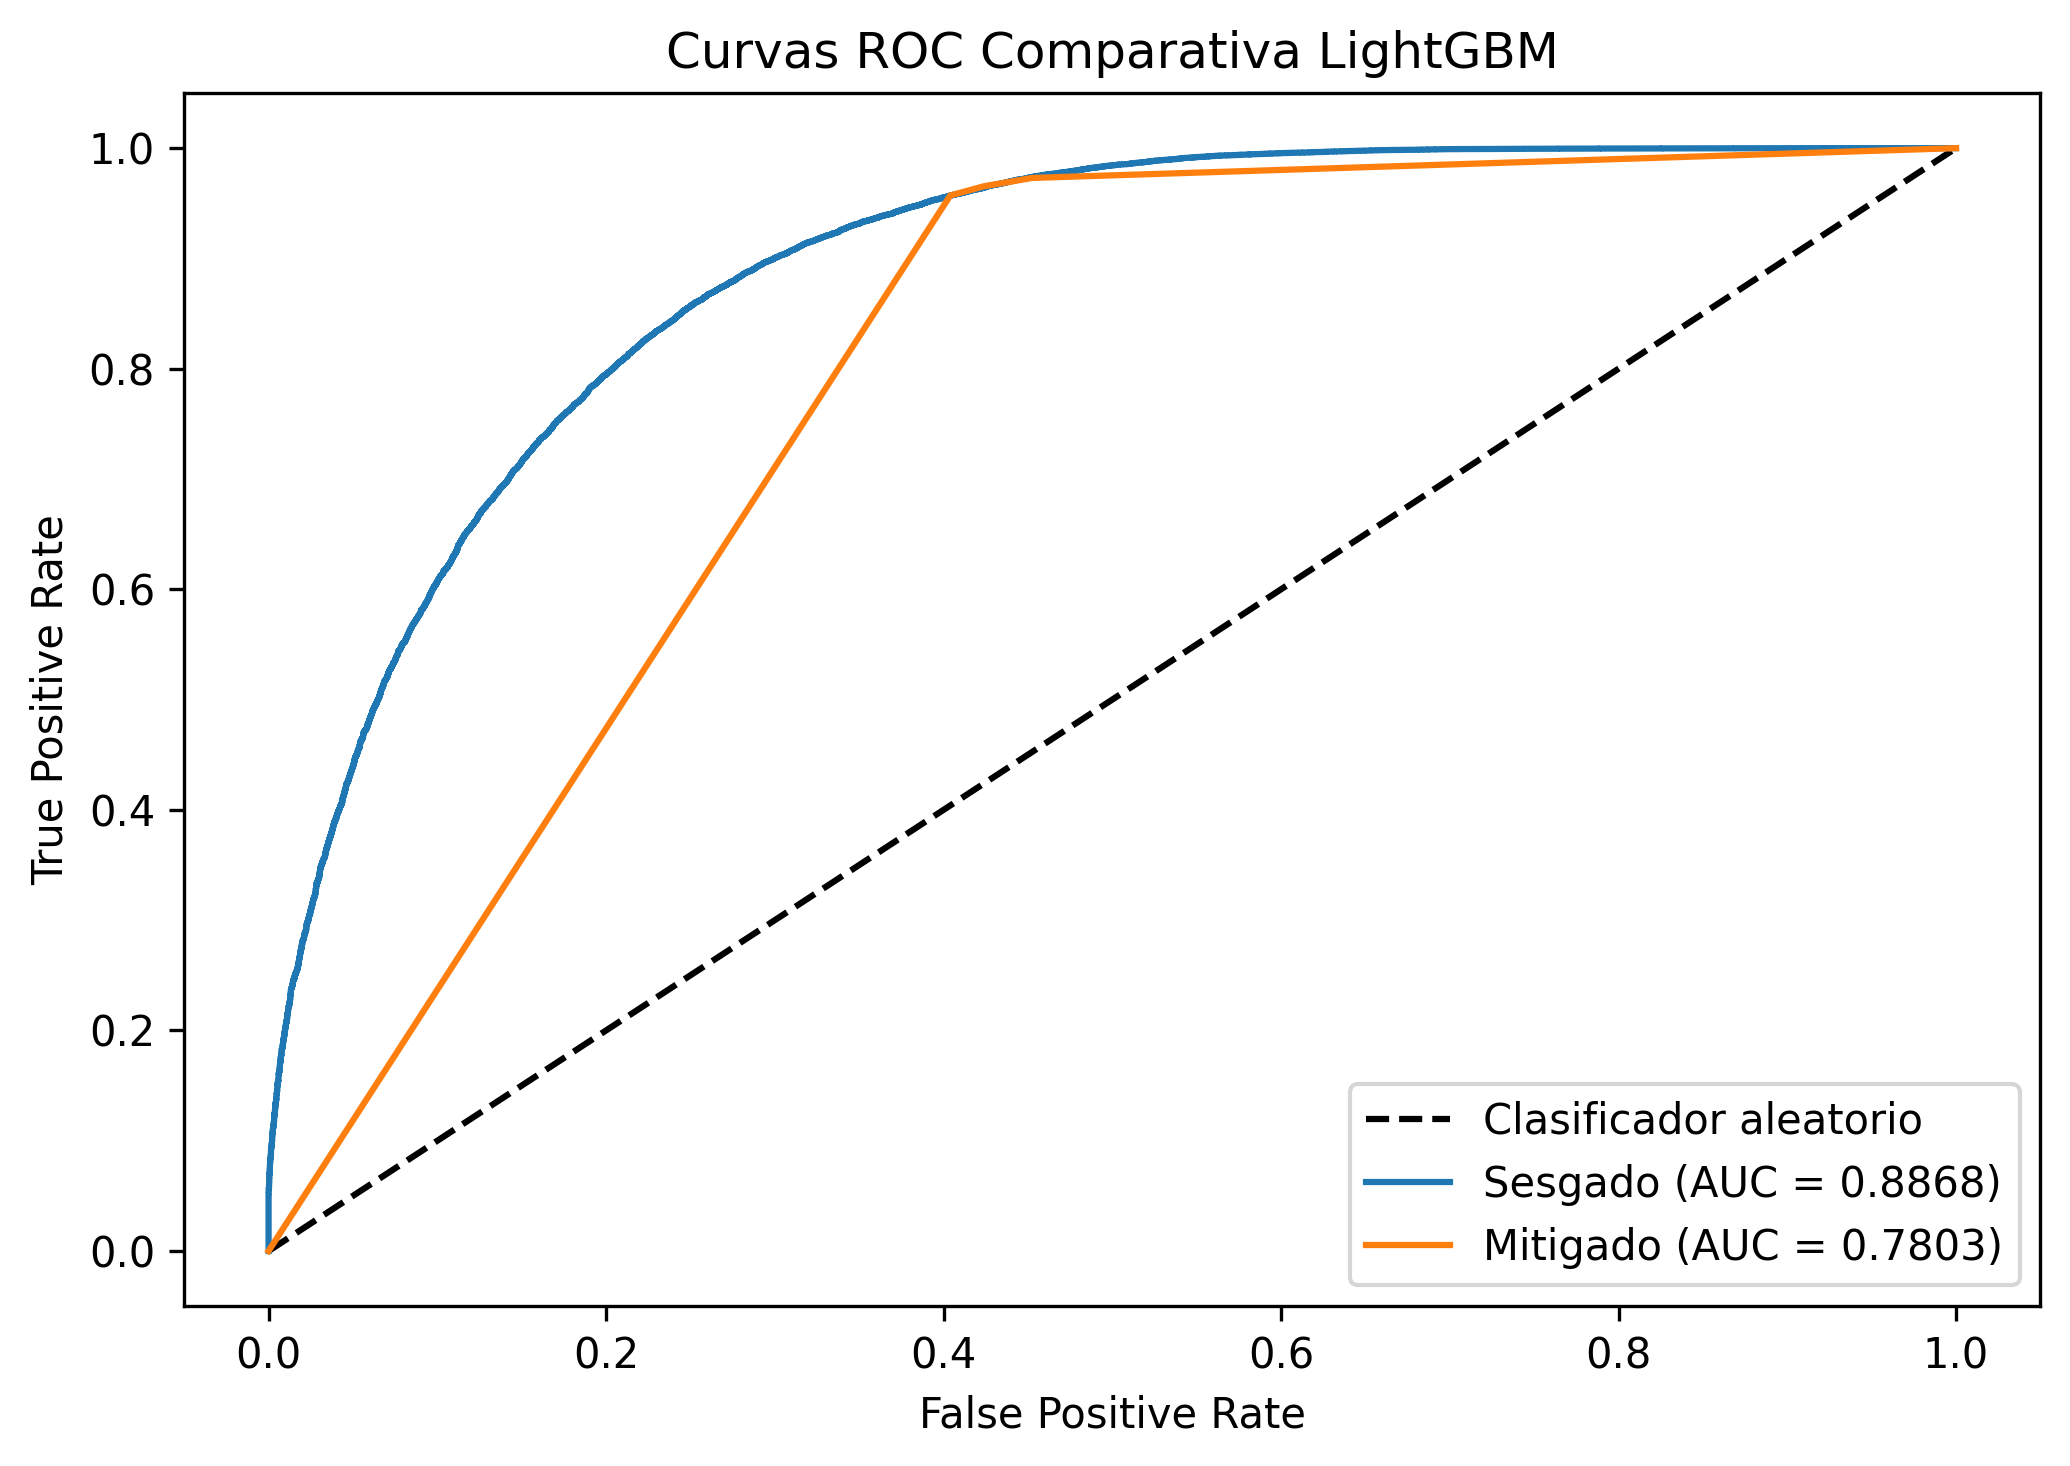
\includegraphics[width=0.6\textwidth]{../outputs/images/curva_roc_sesgos.png}
\caption{Curvas ROC comparativas --- LightGBM sesgado (AUC = 0{,}8868) vs.\ mitigado
(AUC = 0{,}7803). La caída es el coste directo de imponer la restricción \texttt{EqualizedOdds}.}
\label{fig:roc_comparativo}
\end{figure}
\newpage
La curva ROC del mitigado muestra un comportamiento especialmente distinto en la zona de bajo
FPR (0{,}0--0{,}4), donde el modelo sesgado despega rápidamente hacia TPR altos mientras el mitigado
sube de forma más gradual. Esto indica que el modelo mitigado es menos capaz de identificar
aprobaciones reales con alta precisión, pero lo hace de forma más equitativa entre grupos.

\begin{figure}[H]
\centering
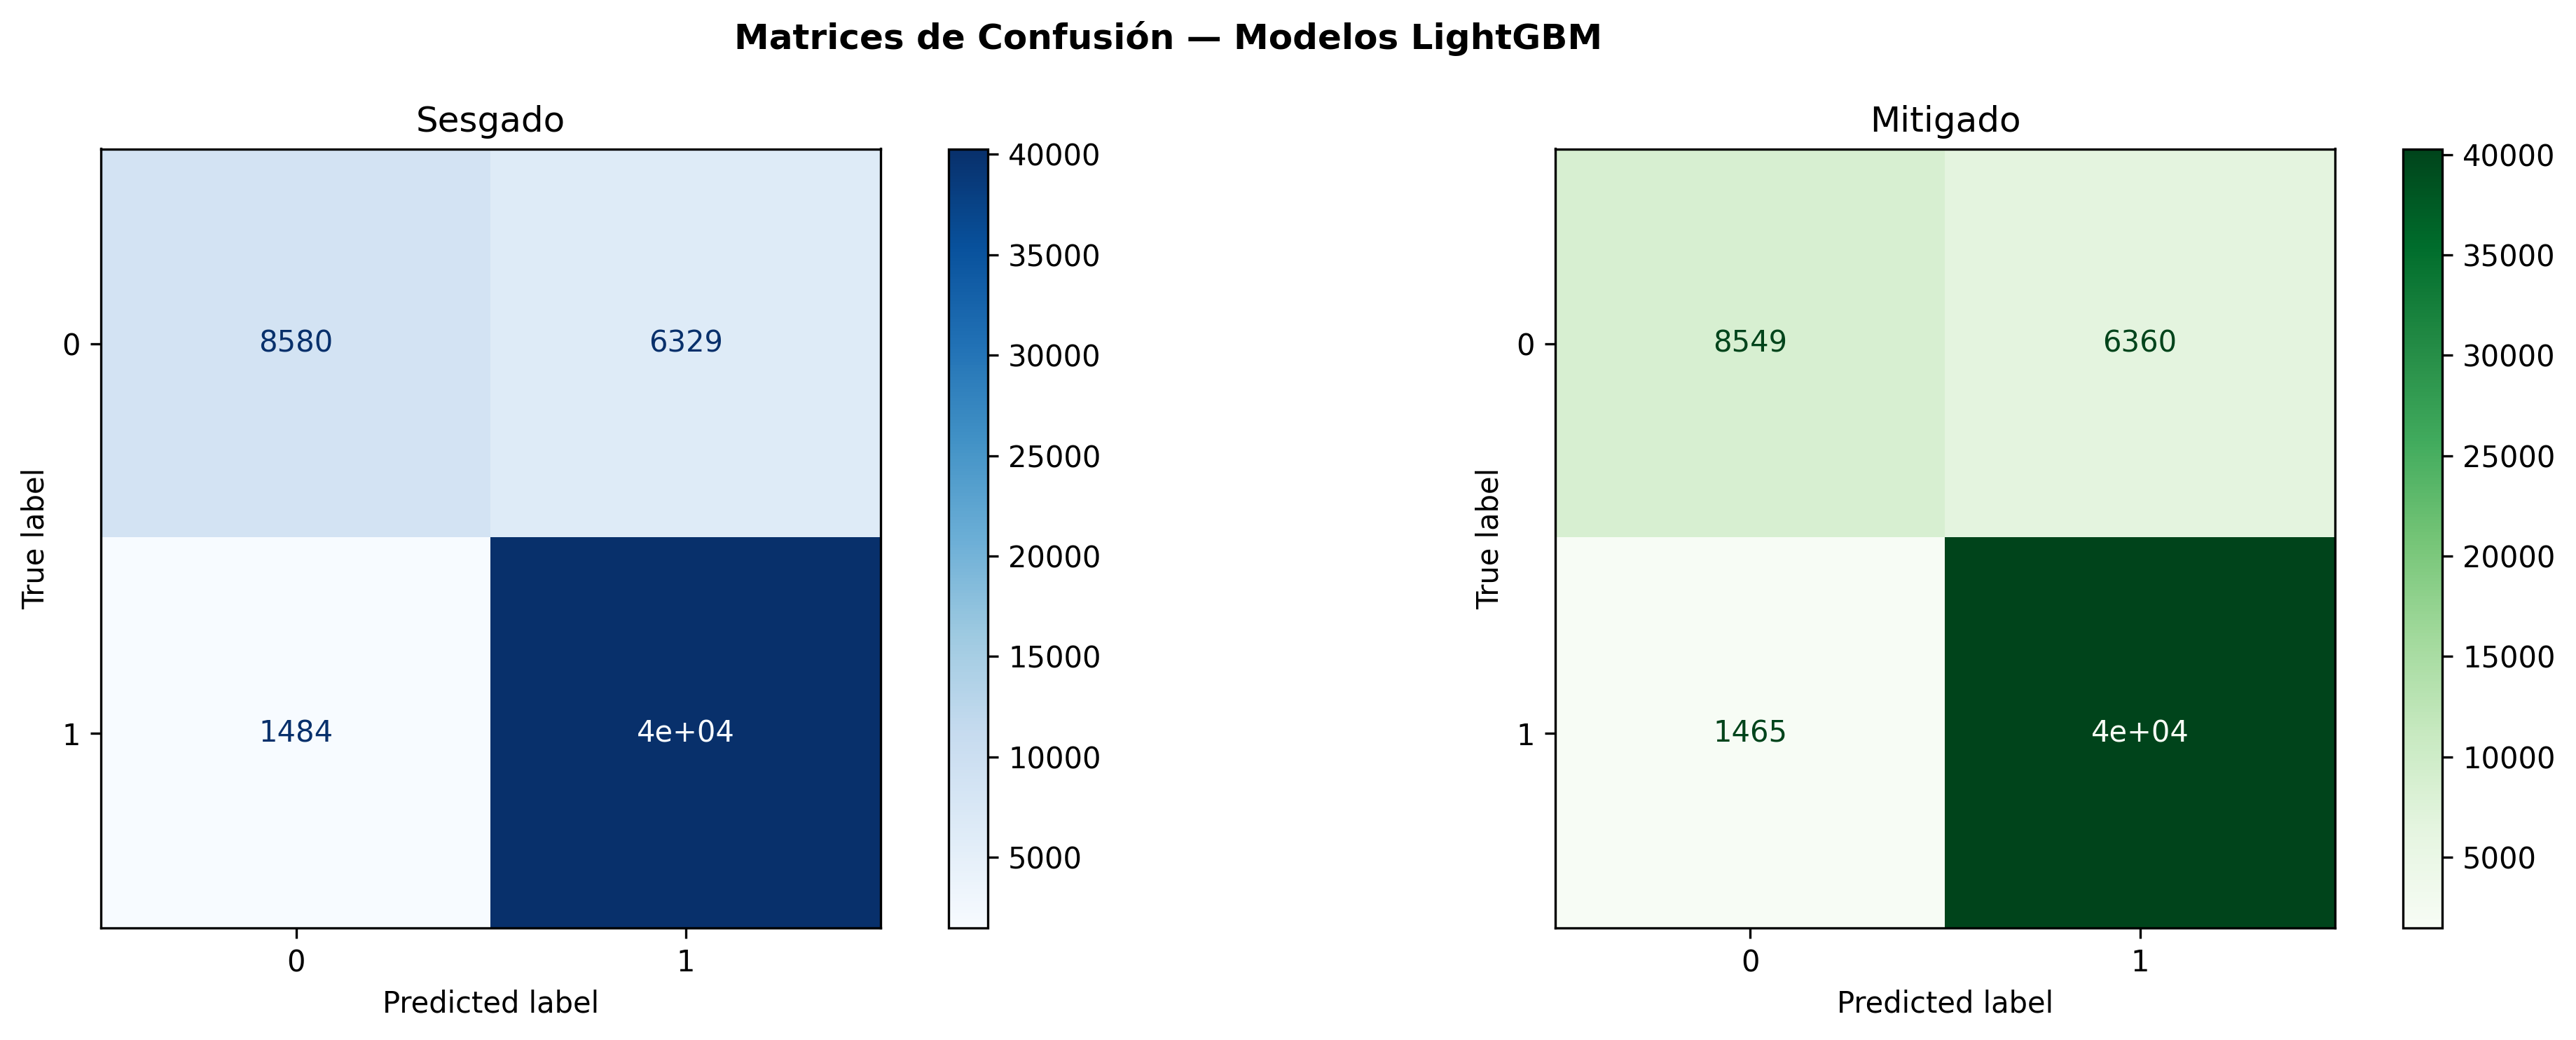
\includegraphics[width=\textwidth]{../outputs/images/matriz_confusion_sesgos.png}
\caption{Matrices de confusión comparativas --- LightGBM sesgado (izquierda) vs.\ mitigado
(derecha). Las diferencias absolutas son mínimas: el coste de la equidad no recae sobre la calidad
de las decisiones individuales sino sobre la capacidad de ordenar probabilidades.}
\label{fig:cm_comparativo}
\end{figure}

Las matrices de confusión revelan que, a pesar de la caída en ROC-AUC, el rendimiento en
predicción directa apenas varía. El modelo sesgado comete 1.484 falsos negativos y 6.329 falsos
positivos; el mitigado presenta 1.455 falsos negativos ($-29$) y 6.354 falsos positivos ($+25$).
Esto ilustra que Accuracy y F1 no son métricas suficientes para detectar sesgo: dos modelos pueden
tener matrices de confusión casi idénticas y diferir significativamente en equidad entre subgrupos.

\subsubsection{Análisis de Fairness comparativo}

\begin{figure}[H]
\centering
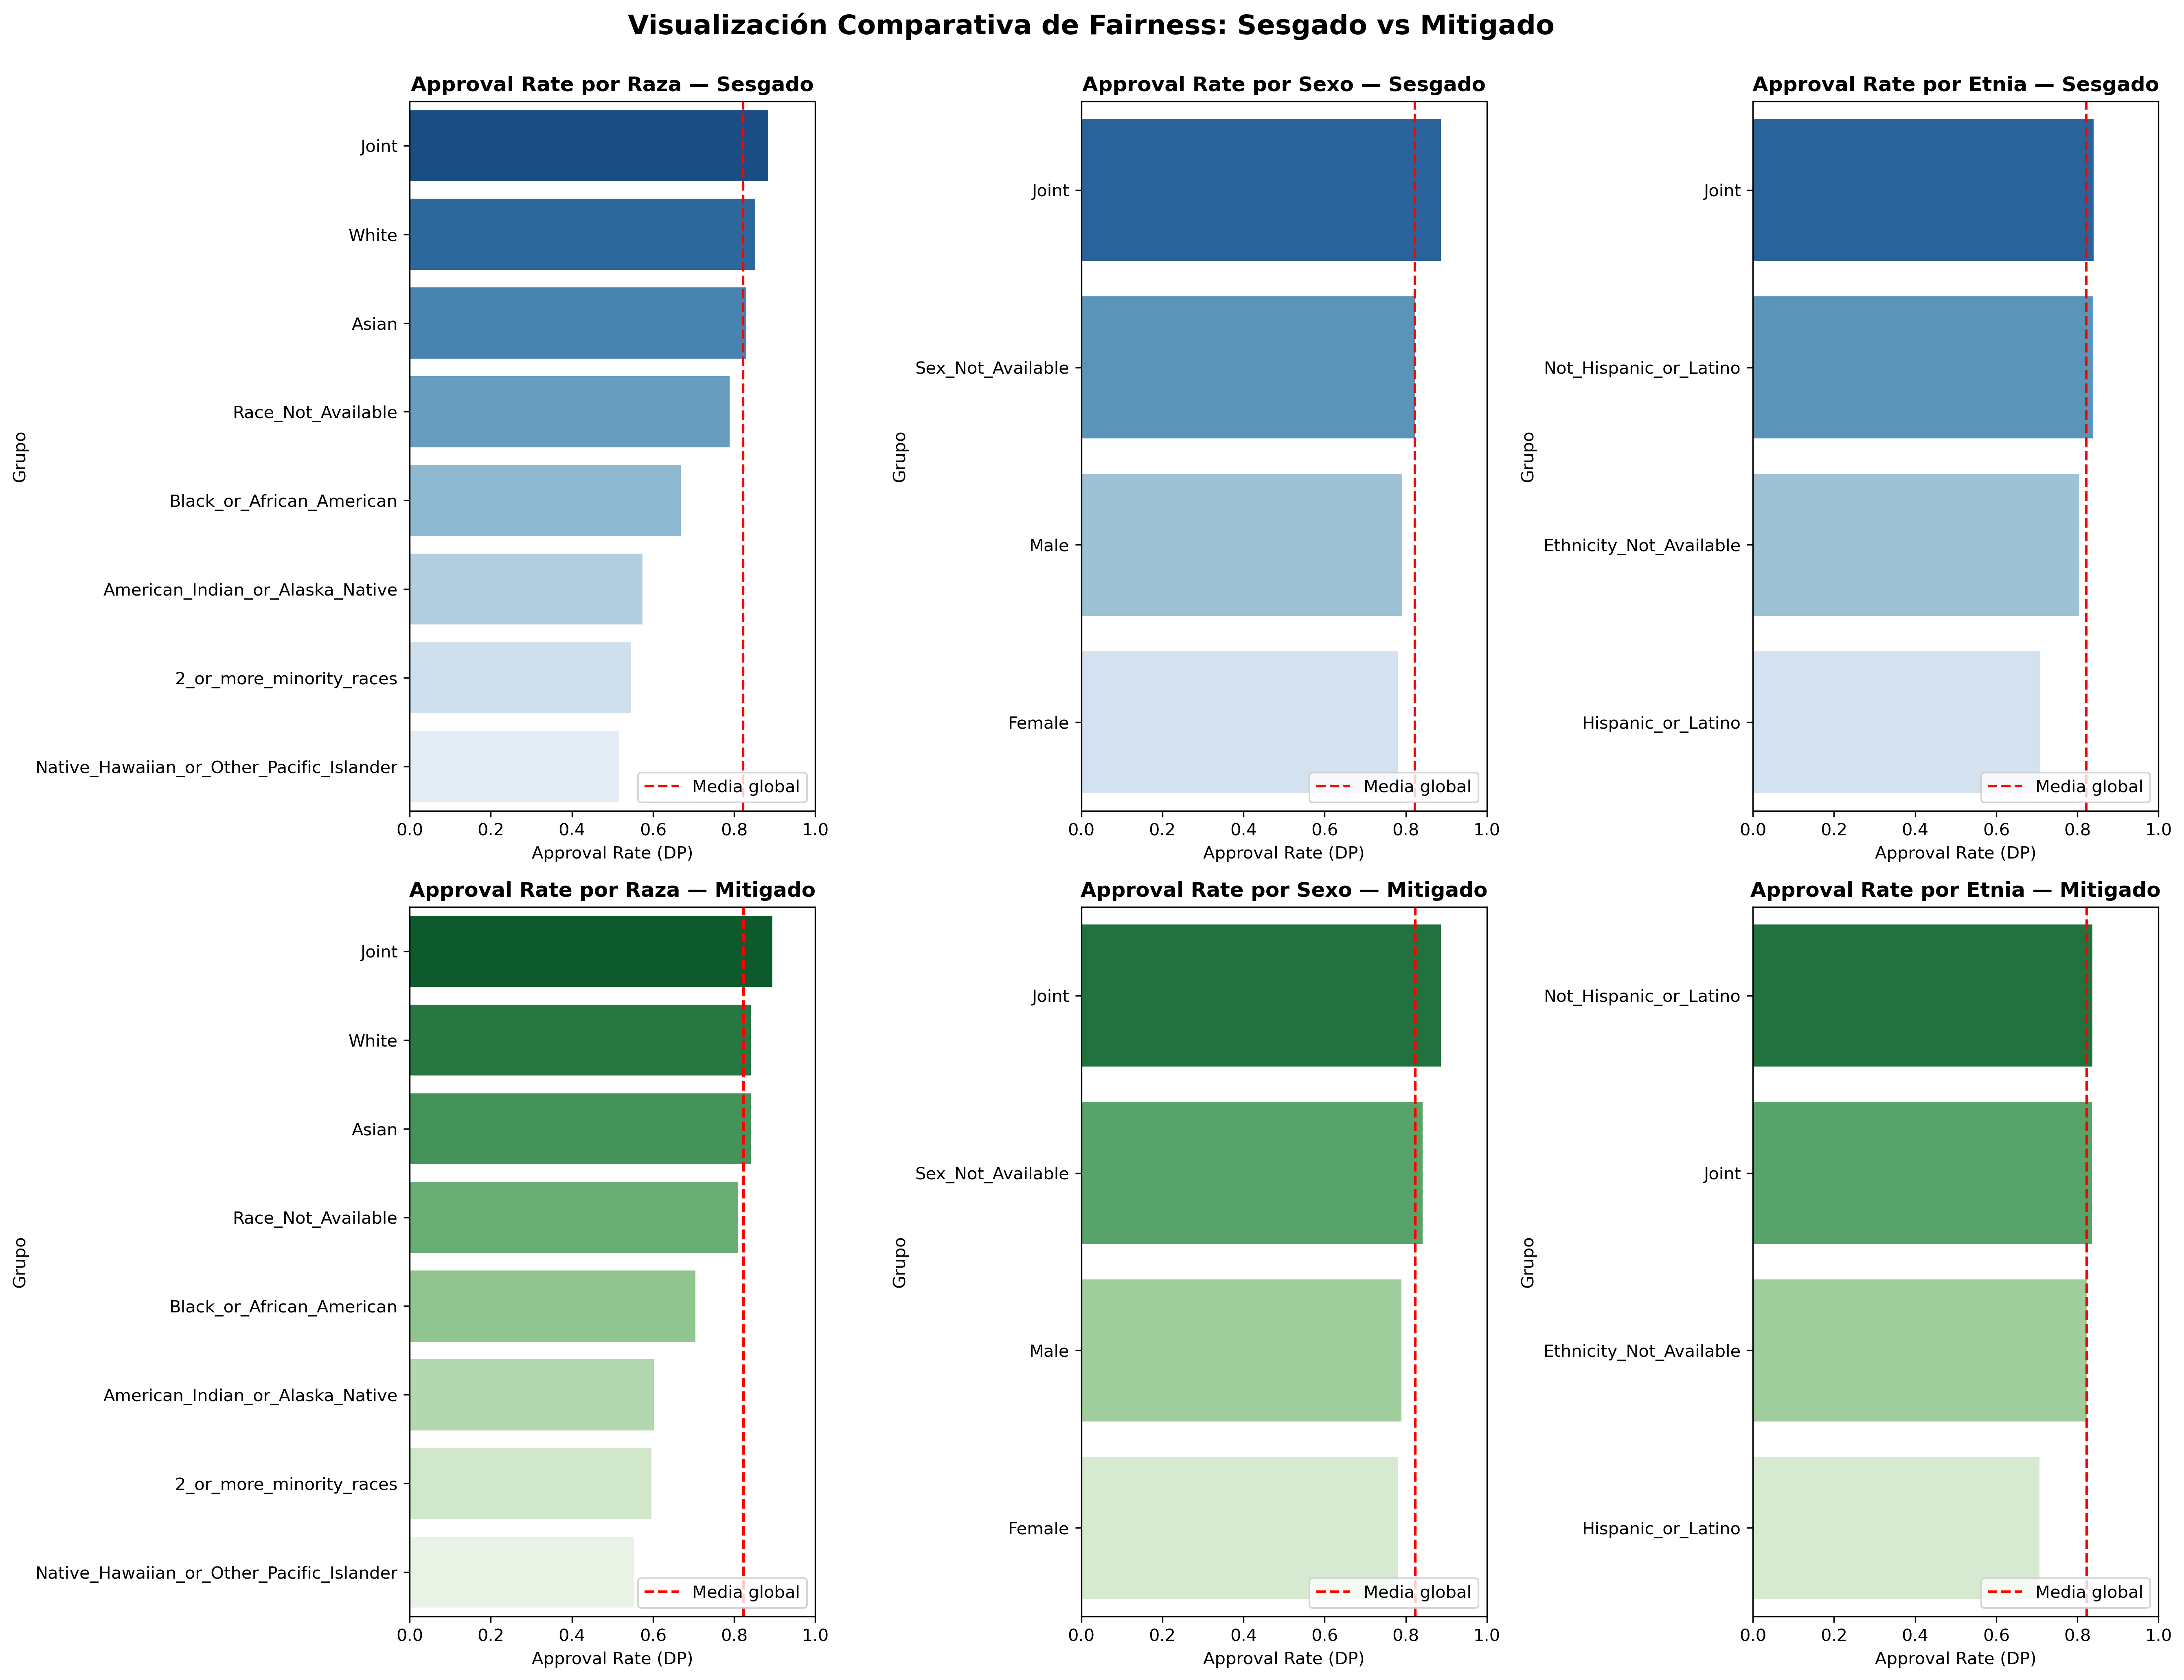
\includegraphics[width=\textwidth]{../outputs/images/fairness_sesgos.png}
\caption{Visualización comparativa de fairness (2$\times$3): sesgado (fila superior) vs.\ mitigado
(fila inferior) para raza, sexo y etnia. Las barras de los grupos minoritarios se desplazan hacia
la derecha en el panel inferior, reduciendo la distancia a la media global.}
\label{fig:fairness_comparativo}
\end{figure}

\begin{table}[ht]
\centering
\caption{Métricas de fairness comparativas --- sesgado vs.\ mitigado}
\label{tab:fairness_comparativo}
\small
\begin{tabular}{@{}llcccc@{}}
\toprule
\textbf{Atributo} & \textbf{Grupo} & \multicolumn{2}{c}{\textbf{Approval Rate (DP)}} & \multicolumn{2}{c}{\textbf{TPR}} \\
 & & \textbf{Sesgado} & \textbf{Mitigado} & \textbf{Sesgado} & \textbf{Mitigado} \\ \midrule
\multirow{4}{*}{Raza}
  & White & 85{,}25\% & 84{,}13\% & 0{,}9709 & 0{,}9641 \\
  & Black & 66{,}86\% & 70{,}42\% & 0{,}9189 & 0{,}9474 \\
  & Am. Indian & 57{,}43\% & 60{,}24\% & 0{,}8923 & 0{,}9077 \\
  & \textbf{Brecha (pp)} & \textbf{18{,}39} & \textbf{13{,}71} & --- & --- \\
\midrule
\multirow{2}{*}{Etnia}
  & Not Hispanic & 83{,}92\% & 83{,}69\% & 0{,}9685 & 0{,}9672 \\
  & Hispanic & 70{,}78\% & 70{,}60\% & 0{,}9333 & 0{,}9314 \\
\midrule
\multirow{2}{*}{Sexo}
  & Male & 79{,}16\% & 78{,}96\% & 0{,}9584 & 0{,}9564 \\
  & Female & 78{,}06\% & 78{,}05\% & 0{,}9553 & 0{,}9567 \\
\bottomrule
\end{tabular}
\end{table}
\newpage
\paragraph{Análisis por raza.}

La brecha racial se reduce de 18{,}39 pp a \textbf{13{,}71 pp} ($-4{,}68$ pp). La tasa de
aprobación de personas negras sube del 66{,}86\% al 70{,}42\% (+3{,}56 pp) y la de American
Indian del 57{,}43\% al 60{,}24\% (+2{,}81 pp). Significativamente, la tasa de aprobación de
personas blancas baja ligeramente del 85{,}25\% al 84{,}13\%, lo que refleja el mecanismo de la
restricción \texttt{EqualizedOdds}: nivelar implica ceder algo en el grupo dominante.

\paragraph{Análisis por etnia.}

La mitigación tiene un efecto prácticamente nulo sobre la brecha étnica (13{,}14 pp $\to$
13{,}53 pp, variación de $-0{,}18$ pp en hispanos). Esto pone de manifiesto una limitación
importante: mitigar sobre un único atributo sensible binario (White/no-White) no generaliza
automáticamente a otras dimensiones de desigualdad como la etnia.

\paragraph{Análisis por sexo.}

La mitigación tiene efecto mínimo sobre las disparidades por sexo, que ya eran las más reducidas.
Las tasas de hombres y mujeres permanecen prácticamente inalteradas, lo que tiene sentido: la
restricción se aplicó exclusivamente sobre \texttt{derived\_race\_White}, por lo que el modelo no
recibe presión directa para corregir las disparidades de sexo.

\subsubsection{Análisis SHAP comparativo}

\begin{figure}[H]
\centering
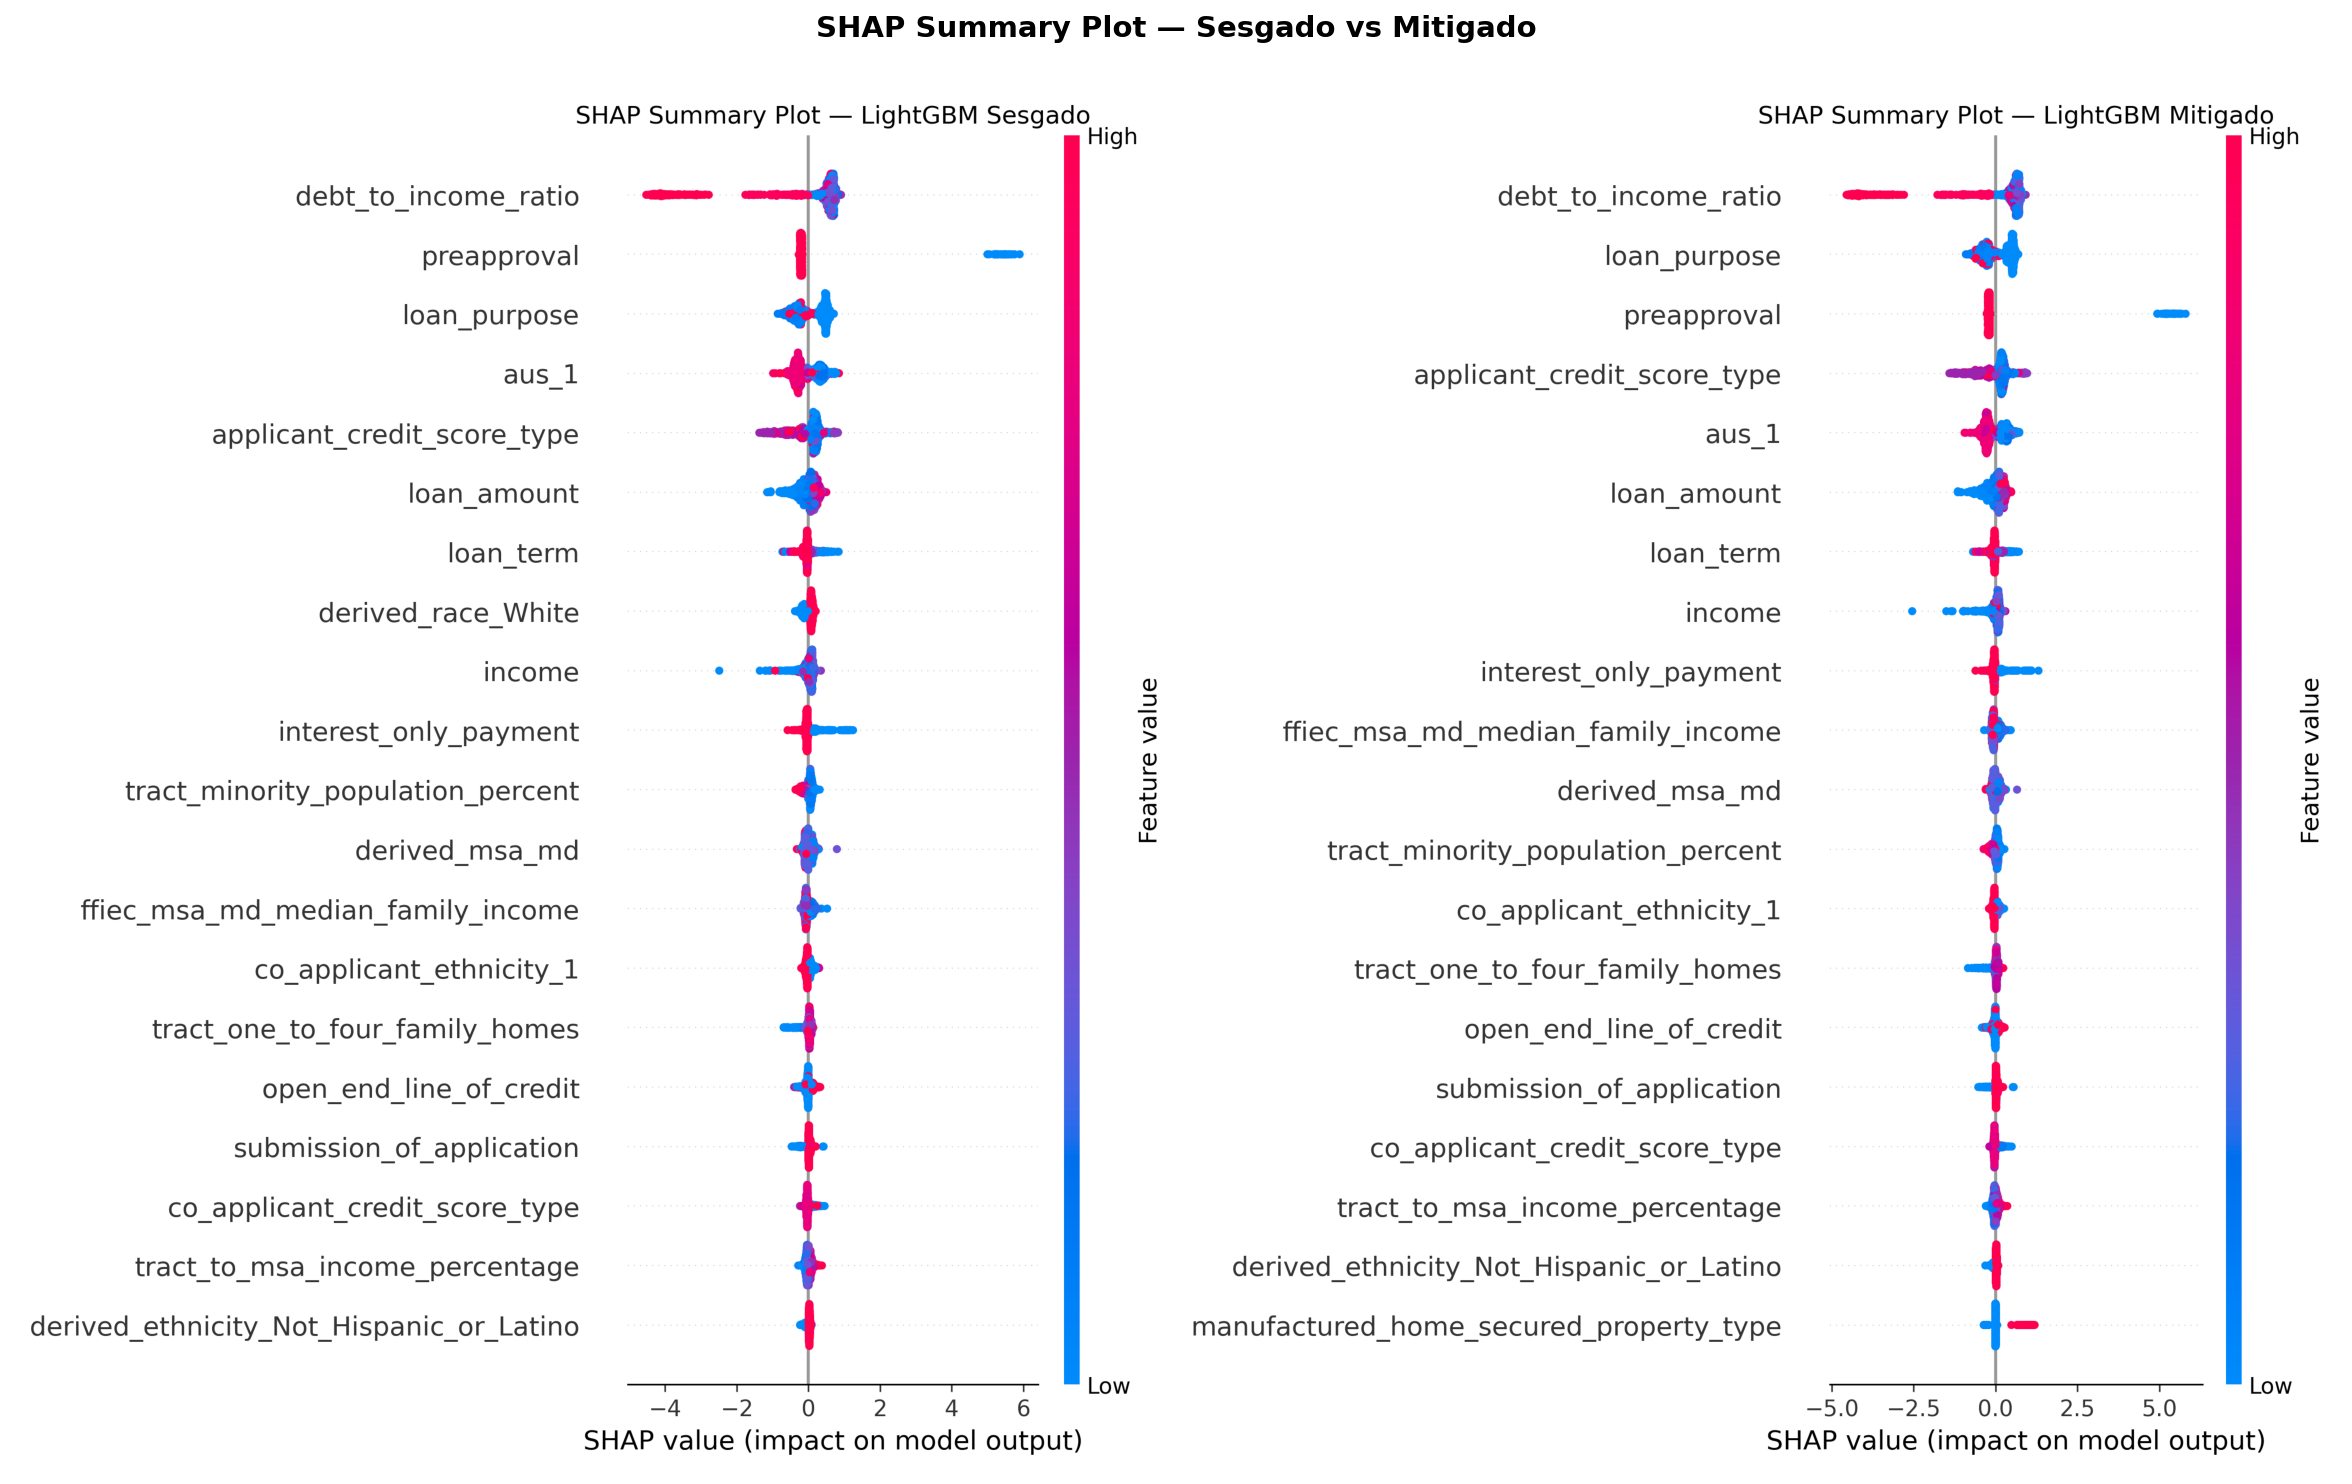
\includegraphics[width=\textwidth]{../outputs/images/shap_summary_comparativo.png}
\caption{SHAP Summary Plot comparativo --- sesgado (izquierda) vs.\ mitigado (derecha).
\texttt{debt\_to\_income\_ratio} mantiene su dominio en ambos modelos. La distribución de puntos
de \texttt{derived\_race\_White} se comprime hacia el centro en el modelo mitigado.}
\label{fig:shap_summary_comp}
\end{figure}

\begin{figure}[H]
\centering
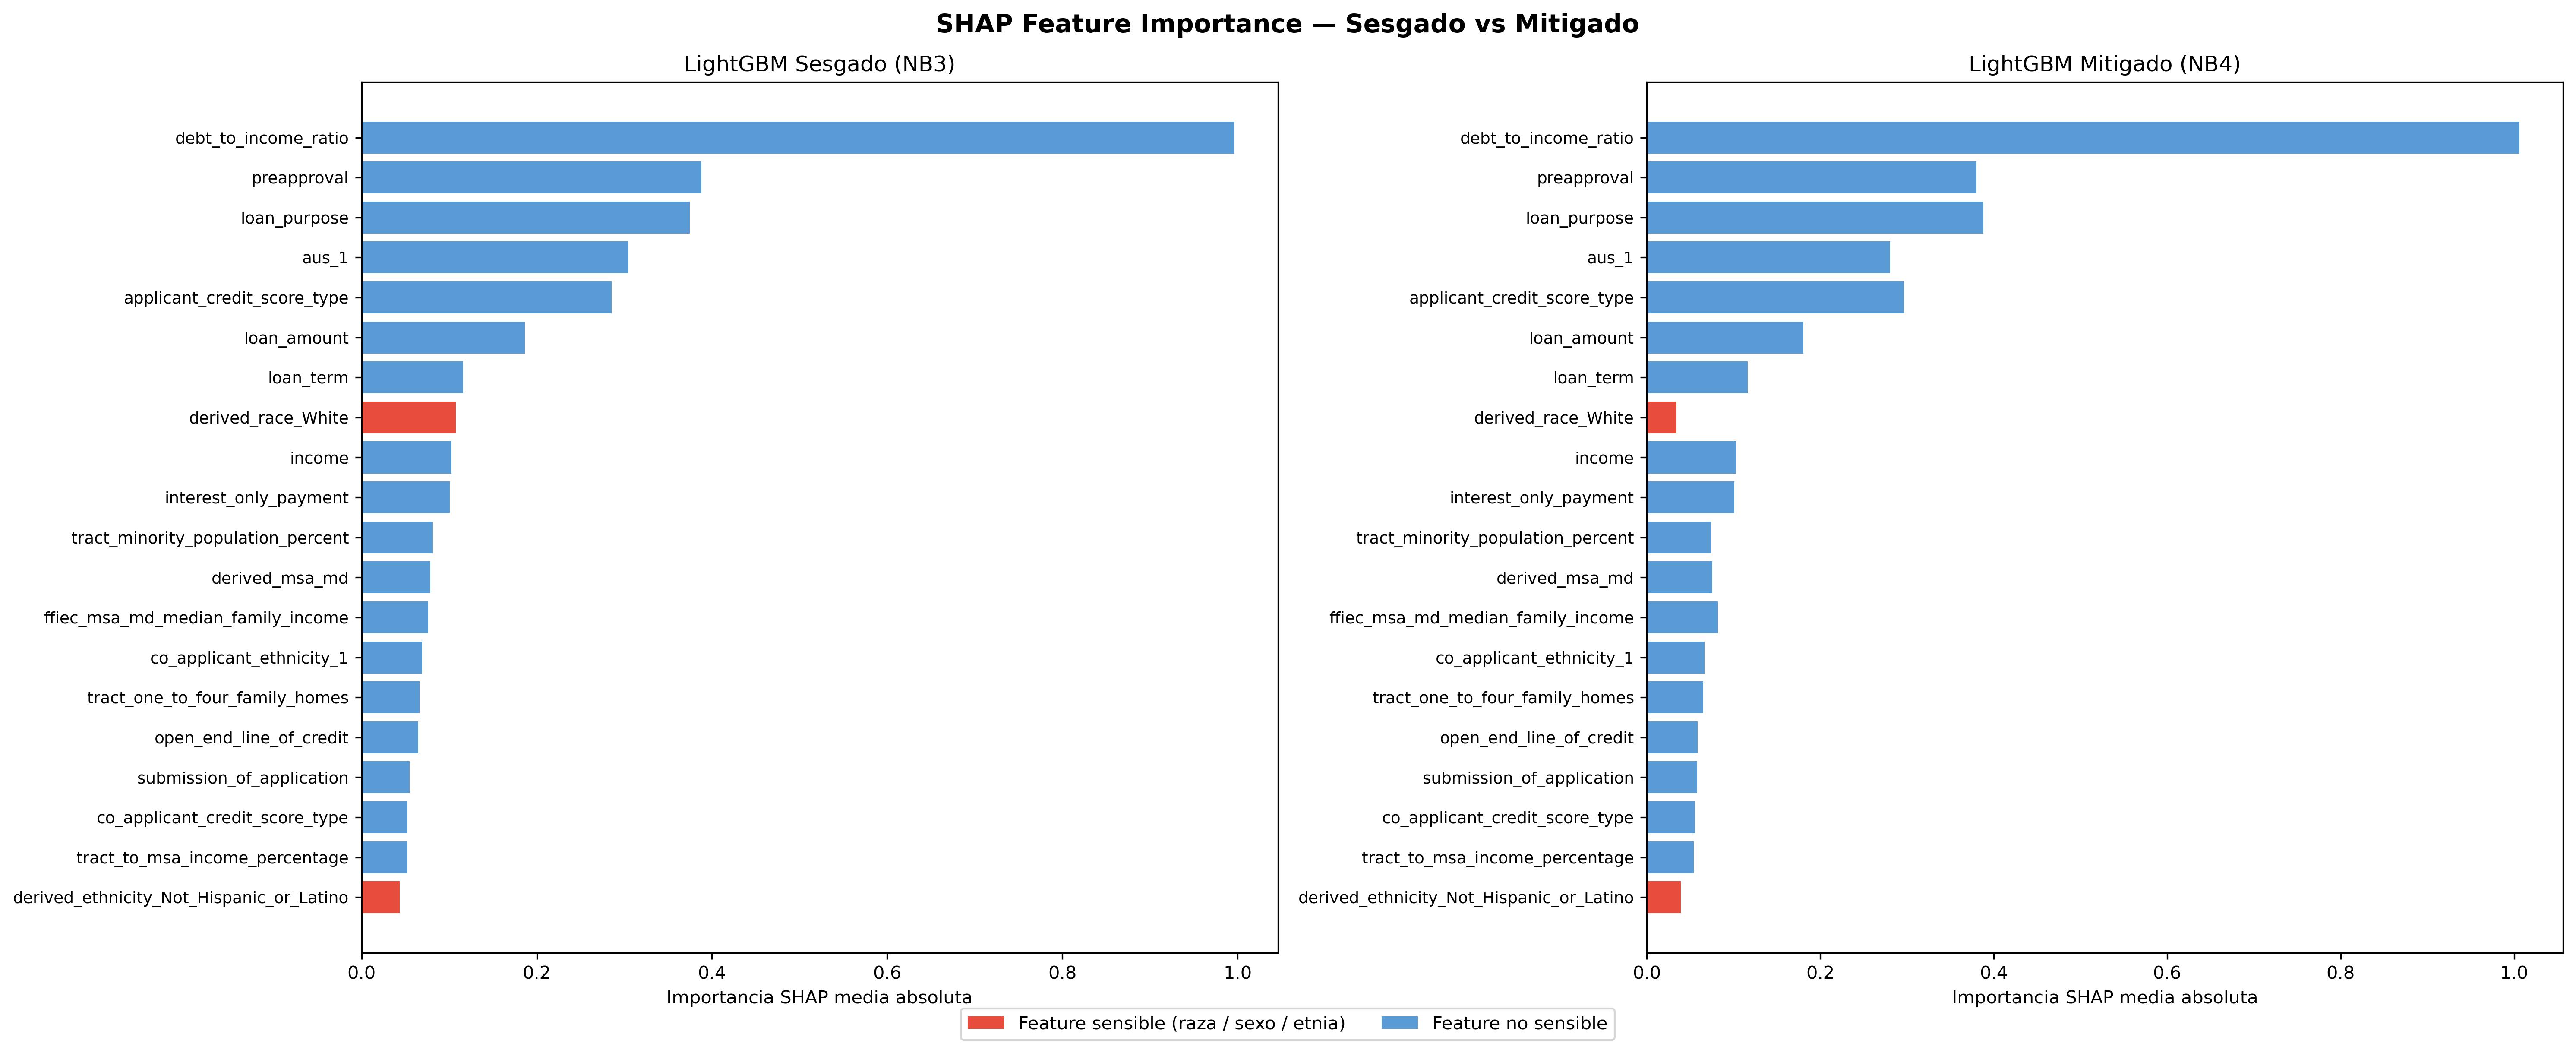
\includegraphics[width=\textwidth]{../outputs/images/shap_bar_comparativo.png}
\caption{SHAP Feature Importance comparativo --- sesgado (izquierda) vs.\ mitigado (derecha).
En rojo, las features sensibles. La barra de \texttt{derived\_race\_White} se reduce
drásticamente tras la mitigación.}
\label{fig:shap_bar_comp}
\end{figure}

El bar plot comparativo (Figura~\ref{fig:shap_bar_comp}) cuantifica con precisión el efecto de
la mitigación: \texttt{derived\_race\_White} reduce su importancia media absoluta de $\sim$0{,}10
a $\sim$0{,}03, cayendo a menos de un tercio. Esta es la evidencia SHAP más directa del
\textit{trade-off} central del proyecto.

Las features estrictamente financieras (\texttt{debt\_to\_income\_ratio}, \texttt{preapproval},
\texttt{loan\_purpose}, \texttt{aus\_1}) mantienen su dominio absoluto en ambos modelos, lo que
confirma que la mitigación no ha distorsionado la lógica económica subyacente sino que ha reducido
específicamente el canal discriminatorio.

\subsubsection{Tabla resumen final y trade-off}

\begin{table}[ht]
\centering
\caption{Tabla resumen final --- Baseline vs.\ LightGBM Sesgado vs.\ LightGBM Mitigado}
\label{tab:resumen_final}
\small
\begin{tabular}{@{}lcccccc@{}}
\toprule
\textbf{Modelo} & \textbf{Accuracy} & \textbf{F1} & \textbf{ROC-AUC} & \textbf{AR White} & \textbf{AR Black} & \textbf{Brecha (pp)} \\ \midrule
Baseline (LR)      & 0{,}7120 & 0{,}7874 & 0{,}7697 & 66{,}85\% & 32{,}29\% & 34{,}56 \\
LightGBM Sesgado   & 0{,}8621 & 0{,}9116 & 0{,}8868 & 85{,}25\% & 66{,}86\% & 18{,}39 \\
\textbf{LightGBM Mitigado} & \textbf{0{,}8622} & \textbf{0{,}9117} & \textbf{0{,}7803} & \textbf{84{,}13\%} & \textbf{70{,}42\%} & \textbf{13{,}71} \\
\bottomrule
\end{tabular}
\end{table}

\begin{figure}[H]
\centering
\includegraphics[width=\textwidth]{../outputs/images/tradeoff_final.png}
\caption{Trade-off rendimiento vs.\ equidad. Izquierda: ROC-AUC de cada modelo.
Derecha: brecha racial (Approval Rate White $-$ Approval Rate Black) en puntos porcentuales.
El modelo mitigado logra la menor brecha racial a costa de una caída en ROC-AUC.}
\label{fig:tradeoff}
\end{figure}

La tabla y el gráfico condensan el recorrido completo del proyecto. El \textbf{baseline} partía de
un rendimiento moderado (ROC-AUC 0{,}7697) con la brecha racial más alta (34{,}56 pp). El
\textbf{LightGBM sesgado} maximiza el rendimiento (ROC-AUC 0{,}8868) pero mantiene una
brecha de 18{,}39 pp, reduciéndola respecto al baseline como efecto secundario de un mejor
ajuste global, no por diseño. El \textbf{LightGBM mitigado} acepta una caída de ROC-AUC hasta
0{,}7803 para reducir la brecha racial a 13{,}71 pp. Accuracy y F1 permanecen prácticamente
inalterados, lo que demuestra que el coste de la equidad no recae sobre la calidad de las
decisiones individuales sino sobre la capacidad de ordenar probabilidades.

En el contexto regulatorio de concesión de hipotecas, donde la \textit{Equal Credit Opportunity Act}
y el \textit{Fair Housing Act} exigen justificación de cada denegación, el modelo mitigado ofrece
el equilibrio más defendible: rendimiento robusto, lógica financiera preservada
(\texttt{debt\_to\_income\_ratio} domina las decisiones) y sesgo racial significativamente reducido.

% ============================================================
\section{Experimentos y resultados}
\label{sec:resultados}
% ============================================================

Esta sección consolida los resultados experimentales obtenidos a lo largo de los tres modelos.
El protocolo de evaluación es común a todos ellos: partición estratificada 80/20, optimización
de hiperparámetros mediante \texttt{GridSearchCV} con validación cruzada de 3 \textit{folds} y
\texttt{roc\_auc} como métrica de búsqueda. Las métricas de rendimiento (Accuracy, F1-Score,
ROC-AUC) se complementan con métricas de \textit{fairness} (\textit{Demographic Parity} y
\textit{Equalized Odds}) calculadas por subgrupo demográfico, dado que en un problema de auditoría
de sesgo las métricas globales son insuficientes por sí solas.

\textbf{Rendimiento.} La Tabla~\ref{tab:resumen_final} recoge la comparativa final de los tres
modelos. El baseline de Regresión Logística alcanza un ROC-AUC de 0{,}7697. Los modelos de
\textit{ensemble} elevan esta cifra por encima de 0{,}88 (Tabla~\ref{tab:comparativa_modelos}),
con LightGBM seleccionado como modelo final (ROC-AUC 0{,}8868). Tras la mitigación, el ROC-AUC
del modelo cae a 0{,}7803, mientras que Accuracy (0{,}8622) y F1-Score (0{,}9117) permanecen
prácticamente inalterados respecto al modelo sesgado.

\textbf{Equidad.} La brecha racial en tasa de aprobación ---diferencia entre personas blancas y
negras--- evoluciona de 34{,}56 pp en el baseline a 18{,}39 pp en el LightGBM sesgado y a
13{,}71 pp en el LightGBM mitigado (Tabla~\ref{tab:fairness_comparativo}). La
Figura~\ref{fig:tradeoff} visualiza el \textit{trade-off} entre ambas dimensiones: el modelo
mitigado logra la menor brecha racial de los tres a costa de la mayor caída de ROC-AUC.

\textbf{Explicabilidad.} El análisis SHAP (Figuras~\ref{fig:shap_bar_lgbm}
y~\ref{fig:shap_bar_comp}) cuantifica el efecto de la mitigación sobre el uso de la raza: la
importancia media absoluta de \texttt{derived\_race\_White} pasa de $\sim$0{,}10 (posición 8 del
ranking) en el modelo sesgado a $\sim$0{,}03 en el mitigado. Las \textit{features} financieras
(\texttt{debt\_to\_income\_ratio}, \texttt{preapproval}, \texttt{loan\_purpose}, \texttt{aus\_1})
mantienen su dominio en ambos modelos.

% ============================================================
\section{Discusión}
\label{sec:discusion}
% ============================================================

\textbf{Interpretación de los resultados en el contexto del problema.} El hallazgo central del
trabajo es que el sesgo racial no es un artefacto de un modelo concreto sino una propiedad
estructural de los datos: ya el baseline ---un modelo lineal simple--- reproduce una brecha de
34{,}56 pp. El LightGBM, pese a reducir esa cifra a 18{,}39 pp, lo hace como efecto colateral de
un mejor ajuste global y no por un tratamiento explícito de la equidad; el análisis SHAP confirma
que el modelo aprende a usar \texttt{derived\_race\_White} como señal predictiva activa. Esto
ilustra empíricamente la tesis de Barocas y Selbst \cite{barocas2016}: un modelo discrimina aunque
ningún desarrollador lo programe para ello, simplemente al optimizar una función de pérdida sobre
datos que reflejan desigualdades históricas.

\textbf{El trade-off rendimiento--equidad.} La mitigación con \texttt{ExponentiatedGradient} reduce
la brecha racial a 13{,}71 pp, pero a costa de una caída de ROC-AUC de $\sim$10{,}6 pp. Es
fundamental interpretar correctamente este coste: Accuracy y F1-Score apenas varían, y las matrices
de confusión de los modelos sesgado y mitigado son casi idénticas. La pérdida no está en la calidad
de las decisiones binarias individuales sino en la capacidad de \textit{ordenar} probabilidades
---precisamente la dimensión sobre la que actúa la restricción \textit{Equalized Odds}. Este
resultado conecta con la imposibilidad formal demostrada por Kleinberg et al.\ \cite{kleinberg2017}:
no existe un modelo que sea simultáneamente óptimo en discriminación y en equidad de tasas de error,
por lo que la elección del punto de operación es una decisión de diseño con implicaciones éticas,
no un problema puramente técnico.

\textbf{Análisis crítico de las limitaciones.} La limitación más relevante es que la restricción de
\textit{fairness} se aplicó sobre un único atributo sensible binario (\texttt{derived\_race\_White}).
Los resultados muestran que esta mitigación es selectiva: reduce la brecha racial pero deja
prácticamente intactas las brechas por etnia ($-0{,}18$ pp en hispanos) y por sexo. Mitigar una
dimensión de desigualdad no generaliza automáticamente a las demás. Una segunda limitación es la
propia naturaleza del dataset HMDA: registra la decisión del banco, no la solvencia real del
solicitante, por lo que el modelo aprende a replicar las decisiones humanas históricas ---incluido
su sesgo--- y no una noción objetiva de riesgo crediticio. Por último, \texttt{ExponentiatedGradient}
produce un clasificador aleatorizado, lo que introduce una variabilidad que conviene tener presente
en un despliegue real.

\textbf{Implicaciones éticas, sociales y legales.} En el marco de la \textit{Equal Credit Opportunity
Act} y el \textit{Fair Housing Act}, un modelo con una brecha racial de 18{,}39 pp sería difícilmente
defendible ante un auditor regulatorio. El modelo mitigado, con 13{,}71 pp y una importancia SHAP de
la raza reducida a un tercio, ofrece un punto de operación más justificable, aunque la brecha residual
sigue siendo sustancial: la mitigación algorítmica reduce el sesgo pero no lo elimina. Esto sugiere
que las técnicas de \textit{fairness} deben entenderse como una herramienta de reducción de daño
dentro de un proceso más amplio de auditoría y supervisión humana, y no como una solución completa
y automática al problema de la discriminación crediticia.

\newpage
% ============================================================
\section{Conclusiones}
\label{sec:conclusiones}
% ============================================================

\begin{itemize}

    \item \textbf{Sesgo estructural en los datos:} El EDA revela disparidades demográficas en
    las tasas de aprobación antes de cualquier modelado. La brecha racial de 34{,}56 pp entre
    personas blancas y negras en el baseline evidencia que los datos HMDA reflejan desigualdades
    históricas en el acceso al crédito hipotecario, no simplemente diferencias en el perfil financiero.
    La correlación positiva de \texttt{derived\_race\_White} con la aprobación ($+0{,}09$) en
    la matriz de correlación post-preprocesamiento anticipa el sesgo que los modelos amplificarán.

    \item \textbf{Capacidad predictiva de LightGBM:} La selección de LightGBM sobre Gradient
    Boosting, XGBoost y Random Forest está justificada por su combinación óptima de rendimiento
    (ROC-AUC 0{,}8868, prácticamente idéntico al GB 0{,}8871) y eficiencia computacional
    (1{,}90 s frente a $\sim$320 s del GB). Esta diferencia de dos órdenes de magnitud es
    especialmente relevante para el proceso iterativo de \texttt{ExponentiatedGradient}.

    \item \textbf{El acceso a atributos sensibles amplifica el sesgo:} Al comparar el baseline
    (Regresión Logística, modelo lineal simple sin restricciones de equidad) con el LightGBM sesgado
    (modelo de mayor capacidad con acceso a los mismos atributos sensibles), la brecha
    racial pasa de 34{,}56 pp a 18{,}39 pp. Lejos de ser una mejora, esto refleja que el modelo
    de mayor capacidad aprende a usar la raza como señal predictiva: \texttt{derived\_race\_White}
    alcanza la posición 8 en el ranking SHAP con importancia $\sim$0{,}10.

    \item \textbf{Efectividad y límites de la mitigación:} \texttt{ExponentiatedGradient} con
    \texttt{EqualizedOdds} reduce la brecha racial de 18{,}39 pp a 13{,}71 pp ($-4{,}68$ pp)
    y la importancia SHAP de \texttt{derived\_race\_White} de $\sim$0{,}10 a $\sim$0{,}03.
    Sin embargo, la mejora es selectiva: la restricción centrada en el atributo binario
    White/no-White apenas arrastra mejoras para la brecha étnica ($-0{,}18$ pp en hispanos)
    ni para la de sexo. La mitigación algorítmica reduce pero no elimina el sesgo.

    \item \textbf{Trade-off rendimiento--equidad:} El coste principal de la mitigación es la
    caída de ROC-AUC de 0{,}8868 a 0{,}7803 ($-10{,}65$ pp). Accuracy y F1 permanecen
    prácticamente inalterados (diferencias $<0{,}001$), lo que demuestra que la equidad se
    obtiene a expensas del poder discriminativo en el ordenamiento de probabilidades, no de
    la calidad de las predicciones binarias. Las matrices de confusión son casi idénticas entre
    ambos modelos.

    \item \textbf{Lógica financiera preservada:} El análisis SHAP confirma que
    \texttt{debt\_to\_income\_ratio}, \texttt{preapproval}, \texttt{loan\_purpose} y \texttt{aus\_1}
    mantienen su dominio absoluto en ambos modelos. La mitigación no distorsiona la lógica
    económica del modelo sino que reduce específicamente el canal discriminatorio asociado a
    la raza.

    \item \textbf{Limitaciones y trabajo futuro:} La principal limitación es que la restricción
    se aplicó sobre un único atributo sensible binario (\texttt{derived\_race\_White}), sin
    mejoras significativas para etnia o sexo. Como líneas de mejora se propone: (a) aplicar
    restricciones simultáneas sobre múltiples atributos sensibles, (b) explorar otras técnicas
    de mitigación (\texttt{GridSearch} de \texttt{ThresholdOptimizer}, técnicas de
    preprocesamiento como \textit{reweighing}), y (c) evaluar el impacto en subgrupos
    interseccionales (e.g., mujeres negras hispanas). Desde el punto de vista regulatorio, el
    modelo mitigado es el más defendible bajo la \textit{Equal Credit Opportunity Act} y el
    \textit{Fair Housing Act}, aunque la brecha racial residual de 13{,}71 pp sigue siendo
    sustancial y requeriría justificación ante un auditor.

\end{itemize}

\newpage
% ============================================================
\begin{thebibliography}{9}
% ============================================================

\bibitem{agarwal2018}
Agarwal, A., Beygelzimer, A., Dudík, M., Langford, J., \& Wallach, H. (2018).
A Reductions Approach to Fair Classification.
\textit{Proceedings of the 35th International Conference on Machine Learning (ICML)},
PMLR 80, 60--69.

\bibitem{hardt2016}
Hardt, M., Price, E., \& Srebro, N. (2016).
Equality of Opportunity in Supervised Learning.
\textit{Advances in Neural Information Processing Systems (NeurIPS)}, 29, 3315--3323.

\bibitem{lundberg2017}
Lundberg, S. M., \& Lee, S.-I. (2017).
A Unified Approach to Interpreting Model Predictions.
\textit{Advances in Neural Information Processing Systems (NeurIPS)}, 30, 4765--4774.

\bibitem{ke2017}
Ke, G., Meng, Q., Finley, T., Wang, T., Chen, W., Ma, W., Ye, Q., \& Liu, T.-Y. (2017).
LightGBM: A Highly Efficient Gradient Boosting Decision Tree.
\textit{Advances in Neural Information Processing Systems (NeurIPS)}, 30, 3146--3154.

\bibitem{barocas2016}
Barocas, S., \& Selbst, A. D. (2016).
Big Data's Disparate Impact.
\textit{California Law Review}, 104(3), 671--732.

\bibitem{kleinberg2017}
Kleinberg, J., Mullainathan, S., \& Raghavan, M. (2017).
Inherent Trade-Offs in the Fair Determination of Risk Scores.
\textit{Proceedings of the 8th Innovations in Theoretical Computer Science Conference (ITCS)},
43:1--43:23.

\bibitem{mehrabi2021}
Mehrabi, N., Morstatter, F., Saxena, N., Lerman, K., \& Galstyan, A. (2021).
A Survey on Bias and Fairness in Machine Learning.
\textit{ACM Computing Surveys}, 54(6), 1--35.

\bibitem{bird2020}
Bird, S., Dudík, M., Edgar, R., Horn, B., Lutz, R., Milan, V., Sameki, M., Wallach, H.,
\& Walker, K. (2020).
Fairlearn: A Toolkit for Assessing and Improving Fairness in AI.
\textit{Microsoft Technical Report}, MSR-TR-2020-32.

\end{thebibliography}

% ============================================================
\section{Repositorio del código}
% ============================================================

El código fuente completo del proyecto (los cuatro notebooks, los datos y los modelos entrenados)
está disponible en el repositorio público de GitHub:

\begin{center}
\url{https://github.com/jcm204/aa-proyecto-hmda-ny}
\end{center}

\noindent El repositorio incluye un \texttt{README.md} con instrucciones de instalación y ejecución,
un archivo \texttt{requirements.txt} con las dependencias exactas, y los notebooks organizados de
forma secuencial. Todas las semillas aleatorias están fijadas (\texttt{RANDOM\_STATE = 42}) para
garantizar la reproducibilidad de los resultados.

\section{Uso de herramientas de IA generativa}
 
Durante el desarrollo del proyecto se ha empleado puntualmente asistencia de IA generativa como
apoyo en la depuración de código y en la revisión de la redacción de la memoria. En todos los casos
el contenido resultante ha sido revisado, comprendido y validado por los miembros del grupo, y
adaptado a los requisitos específicos del trabajo.

\end{document}
